\section{A numerical study of stochastic optimization for large scale optimal transport}
As presented in the last section, Sinkhorn's algorithm has an relatively high computational complexity that can prohibit its utilization in a very large scale setting. With their linear complexity in general, stochastic optimization algorithms offer an attractive alternative to Sinkhorn, provided the problem can be framed as optimization of an empirical or expected risk. In this section, we will quickly present this formulation, and then study and benchmark the algorithms presented for discrete and semi-discrete optimal transport. All the code used for generating the results of this section is available online\footnote{On GitHub, at the URL \url{https://github.com/hugcis/large-scale-optimal-transport}}.

\subsection{Stochastic optimization for OT}

\subsubsection{Stochastic formulation} \label{section:stoch_formulation}
To make it possible using stochastic optimization methods for the OT problems, we frame the dual \eqref{eq:dual} and semi-dual \eqref{eq:semi-dual} optimization problems as maximization of expectations,
\begin{align*}
    W_\varepsilon(\mu, \nu) &= \max_{(u, v)}\ \mathbb{E}_{X, Y}[f_\varepsilon(X, Y, u, v)] \tag{$\mathbb{E}\mathcal{D_\varepsilon}$}\\
    & = \max_{v}\  \mathbb{E}_{X}[h_\varepsilon(X, v)] \tag{$\mathbb{E}\mathcal{S_\varepsilon}$} \label{eq:stoch-semi-dual}
\end{align*}
Where the two independent random variables $X$ and $Y$ are defined on $\mathcal{X}$, $\mathcal{Y}$, follow respectively the distributions $\mu$ and $\nu$, and with the following definitions for $f_\varepsilon$ and $h_\varepsilon$,
\begin{align*}
    \forall \varepsilon > 0,\ f_\varepsilon(x, y, u, v) &= u(x) + v(y) - \varepsilon\exp\left( \dfrac{u(x) + v(y) - c(x, y)}{\varepsilon} \right)\\
    \forall \varepsilon \geq 0,\ h_\varepsilon(x, v) &= \int_\mathcal{Y} v(y)\text{d}\nu(y)  + v^{c, \varepsilon}(y) - \varepsilon
\end{align*}

\subsubsection{Stochastic optimization algorithms} \label{section:stoch-opti-algo}
Three algorithms will be studied for solving the stochastic OT problems. The first is the standard Stochastic Gradient algorithm (SG). It is based on sampling a realization of the random variable in the expected risk ($X$ on our case) and use it as an estimate of the gradient direction for the update of the iterate. 

In the case of problem \eqref{eq:stoch-semi-dual}, Algorithm \ref{alg:sg} shows the details of each step. The + symbol on line 6 corresponds to a gradient ascent since the objective has to be maximized.

\begin{figure}[htb]
    \centering
    \begin{minipage}{.8\linewidth}
    \begin{algorithm}[H]
        \caption{SG algorithm}\label{alg:sg}
        \begin{algorithmic}[1]
            \State Choose initial iterate $v_0$
            \For {$k=0, ...,K$} 
                \State Generate a realization $x_k$ of X
                \State Compute the stochastic vector $\nabla h_\varepsilon(x_k, v_k)$
                \State Choose step size $\alpha_k$
                \State $v_{k+1} \gets v_k + \alpha_k \nabla h_\varepsilon(x_k, v_k)$
            \EndFor
        \end{algorithmic}
    \end{algorithm}
\end{minipage}
\end{figure}


The two other algorithms studied in the report, Stochastic Averaged Gradient (SAG) \cite{schmidt_minimizing_2013} and SAGA \cite{defazio_saga:_2014} belong to the family of gradient aggregation algorithms. These were designed for finite sum objectives (empirical risks), which is only applicable in our case to the discrete optimization problem as we will see further.

The two methods are based on the idea that keeping a history of past gradient in a stochastic context could give better estimate of the real gradient and thus ensure faster convergence. This intuition is verified, because both SAG and SAGA guarantee a $O(1/k)$ convergence rate in the general case and a linear convergence rate in the strongly convex case \cite{schmidt_minimizing_2013,defazio_saga:_2014}(against $O(1/\sqrt{k})$ and $O(1/k)$ respectively for standard SG for a suitable decreasing step size sequence and standard assumptions \cite{nemirovski_robust_2009}), with automatic adaptation to the local strong-convexity of the objective.

Those properties make them very attractive for applications where SG shows its limitation, and \cite{genevay_stochastic_2016} has presented the advantages of using SAG for discrete optimal transport. One major drawbacks of the gradient aggregation algorithms is the fact that all gradients have to be stored at each step of the algorithm, which can be a  strong limitation when working with very large scale problems.

\subsection{Discrete Optimal Transport}

In the case of discrete OT, we recall that $\mu$ and $\nu$ can both be written as finite sums of Diracs, i.e $\mu = \sum_{i=1}^I \mathbf{\mu}_i \delta_{x_i}$ and $\nu = \sum_{j=1}^J \mathbf{\nu}_j \delta_{y_j}$ with $\forall i, x_i \in \mathcal{X} ; \forall j, x_j \in \mathcal{Y}$ and $\mu \in \Sigma_I, \nu \in \Sigma_J$.

\subsubsection{Details of formulation}

We re-write the primal, dual and semi-dual problems with discrete measures for $\varepsilon > 0$: 
\begin{align*}
    W_\varepsilon(\mu, \nu) &= \min_{\bm{\pi}\in \bm{U}_{\mu, \nu}} \sum_{i,j=1}^{I, J}\mathbf{C}_{i,j} \bm{\pi}_{i,j} + \varepsilon\sum_{i,j}\left( \log\dfrac{\bm{\pi}_{i,j}}{\bm{\mu}_i\bm{\nu}_j}-1 \right)\bm{\pi}_{i,j} \tag{$\overline{\mathcal{P}}_\varepsilon$} \\
    &= \max_{(\bm{u}, \bm{v})\in \mathbb{R}^{I}\times\mathbb{R}^{J}} \sum_{i=1}^I \bm{u}_i \bm{\mu}_i + \sum_{j=1}^J \bm{v}_j \bm{\nu}_j - \varepsilon \sum_{i,j}\exp\left( \frac{\bm{u}_i+\bm{v}_j - \bm{C}_{i,j}}{\varepsilon} \right)\bm{\mu}_i\bm{\nu}_j \tag{$\overline{\mathcal{D}}_\varepsilon$}\\
    &= \max_{\bm{v}\in \mathbb{R}^{J}} \overline{H}_\varepsilon(\bm{v}) = \sum_{i=1}^I \overline{h}_\varepsilon(x_i, \bm{v})\bm{\mu}_i \tag{$\overline{\mathcal{S}}_\varepsilon$} \label{eq:semi-dual-discrete}
\end{align*}

Where we have defined 
\begin{align*}
    \overline{h}_\varepsilon(x, \bm{v}) = \sum_{j=1}^J \bm{v}_j \bm{\nu}_j + 
    \begin{cases}
        -\varepsilon\log\left( \sum_{j=1}^J \exp\left(\frac{\bm{v}_j - c(x, y_j)}{\varepsilon}\right)\bm{\nu}_j \right) - \varepsilon & \text{if }\varepsilon > 0,\\
        \min_j (c(x, y_j) - \bm{v}_j) & \text{if }\varepsilon = 0
    \end{cases}
\end{align*}

Equation \eqref{eq:semi-dual-discrete} can be interpreted as an empirical risk associated with the functions $(\overline{h}_\varepsilon(x_i, \cdot))$. We can therefore apply stochastic optimization algorithms on the problem \eqref{eq:semi-dual-discrete}. The gradient to be computed is 

\begin{align*}  
    \nabla_{\bm{v}} \overline{h}_\varepsilon(x, \bm{v})_j = \bm{\nu}_j - \exp\left(\frac{\bm{v}_j - c(x, y_j)}{\varepsilon}\right) \left( \sum_{i=1}^J \exp\left(\frac{\bm{v}_i - c(x, y_i)}{\varepsilon}\right) \right)^{-1}
\end{align*}

\subsubsection{Stochastic algorithms and discrete OT}

As explained in Section \ref{section:stoch-opti-algo}, SAG and SAGA have comparatively better convergence guarantees than SG for minimizing or maximizing strongly convex and non-strongly convex objectives.

Algorithms \ref{alg:sag_discrete} and \ref{alg:saga_discrete} show the pseudo-code implementation of both algorithms in the case of discrete OT. The parameter \texttt{step} designates a learning rate that is usually chosen in accordance with the Lipschitz constant of the function $\overline{H}_\varepsilon$ to be maximized, $L = \max_i \bm{\mu}_i/\varepsilon$. 

\begin{figure}[h]
    \centering
    \begin{minipage}{.8\linewidth}
    \begin{algorithm}[H]
        \caption{SAG algorithm for discrete OT} \label{alg:sag_discrete}
        \begin{algorithmic}[1]
            \State Choose initial iterate $\bm{v}_1$
            \State $\mathbf{avg} \gets 0_J, \mathbf{grad}_i \gets 0_J$
            \State (Note: Gradient can be initialized with a pass of SG)
            \For {$k=1, ...,K$} 
                \State Sample uniformly $i \in \{1, ..., I\}$
                \State $\mathbf{avg} \gets \mathbf{avg} - \frac{1}{I}\mathbf{grad}_i$
                \State $\mathbf{grad}_i \gets \bm{\mu}_i \nabla_v \overline{h}_\varepsilon(x, \bm{v}_k)$
                \State $\mathbf{avg} \gets \mathbf{avg} + \frac{1}{I}\mathbf{grad}_i$
                \State $\bm{v}_{k+1} \gets \bm{v}_k + \texttt{step} * \mathbf{avg}$
            \EndFor
        \end{algorithmic}
    \end{algorithm}
\end{minipage}
\end{figure}

\begin{figure}[h]
    \centering
    \begin{minipage}{.8\linewidth}
    \begin{algorithm}[H]
        \caption{SAGA algorithm for discrete OT}\label{alg:saga_discrete}
        \begin{algorithmic}[1]
            \State Choose initial iterate $\bm{v}_1$
            \State $\mathbf{avg} \gets 0_J, \mathbf{grad}_i \gets 0_J, \mathbf{last\_grad} \gets 0_J$
            \State (Note: Gradient can be initialized with a pass of SG)
            \For {$k=1, ...,K$} 
                \State Sample uniformly $i \in \{1, ..., I\}$
                \State $\mathbf{last\_grad} \gets \mathbf{grad}_i$
                \State $\mathbf{avg} \gets \mathbf{avg} - \frac{1}{I}\mathbf{last\_grad}$
                \State $\mathbf{grad}_i \gets \bm{\mu}_i \nabla_v \overline{h}_\varepsilon(x, \bm{v}_k)$
                \State $\mathbf{avg} \gets \mathbf{avg} + \frac{1}{I}\mathbf{grad}_i$
                \State $\bm{v}_{k+1} \gets \bm{v}_k + \texttt{step} * (\mathbf{grad}_i - \mathbf{last\_grad} + \mathbf{avg})$
            \EndFor
        \end{algorithmic}
    \end{algorithm}
\end{minipage}
\end{figure}

We first evaluate those algorithms on the toy problem of computing the solution to \eqref{eq:primal} for two random discrete measures with support $\{1,..., N\}$. They are obtained by sampling $N$ values from a uniform distribution on $[0, 1]$ twice and normalizing the histograms in order to obtain measures.

\begin{figure}[h]
    \begin{subfigure}{.49\linewidth}
        \centering
        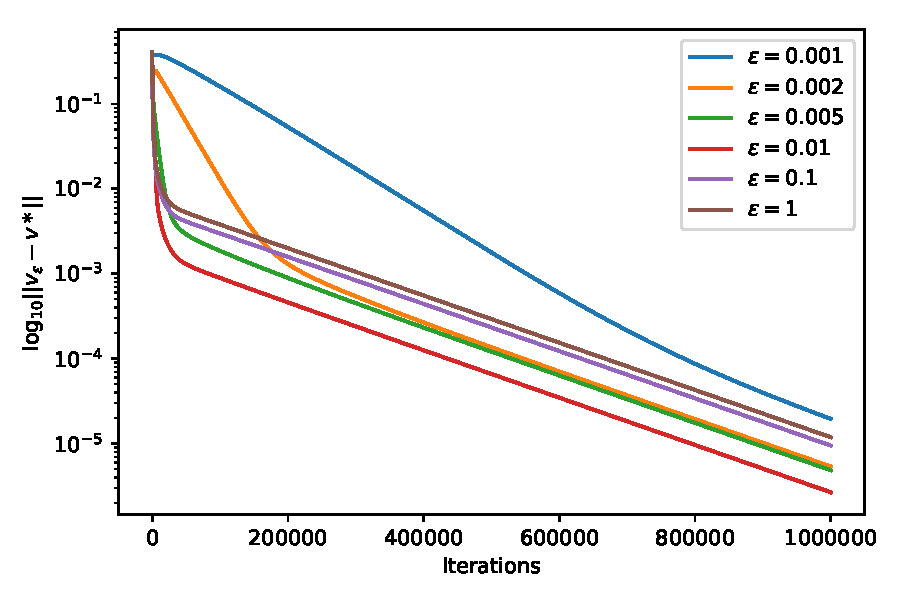
\includegraphics[width=\linewidth]{figures/eps_bench_sag.pdf}
        \caption{Convergence of SAG algorithm for different values of $\varepsilon$.}
    \end{subfigure}
    \begin{subfigure}{.49\linewidth}
        \centering
        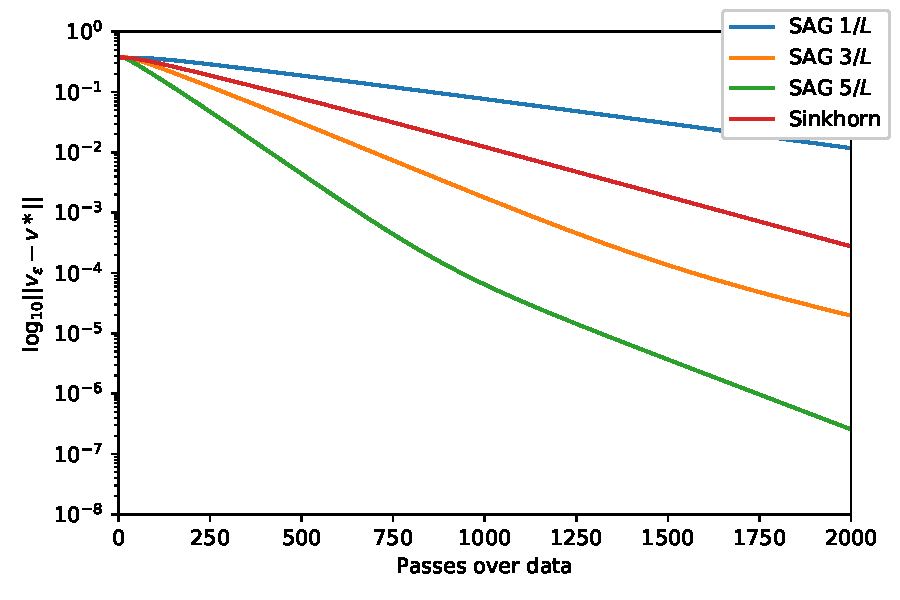
\includegraphics[width=\linewidth]{figures/lr_bench_sag.pdf}
        \caption{Convergence of SAG algorithm for different learning rate and $\varepsilon = 0.001$.}
    \end{subfigure}
    \caption{Convergence of SAG on two randomly generated histograms of size 500. 50 independent runs were averaged.}
\end{figure}

\begin{figure}[h]
    \centering
    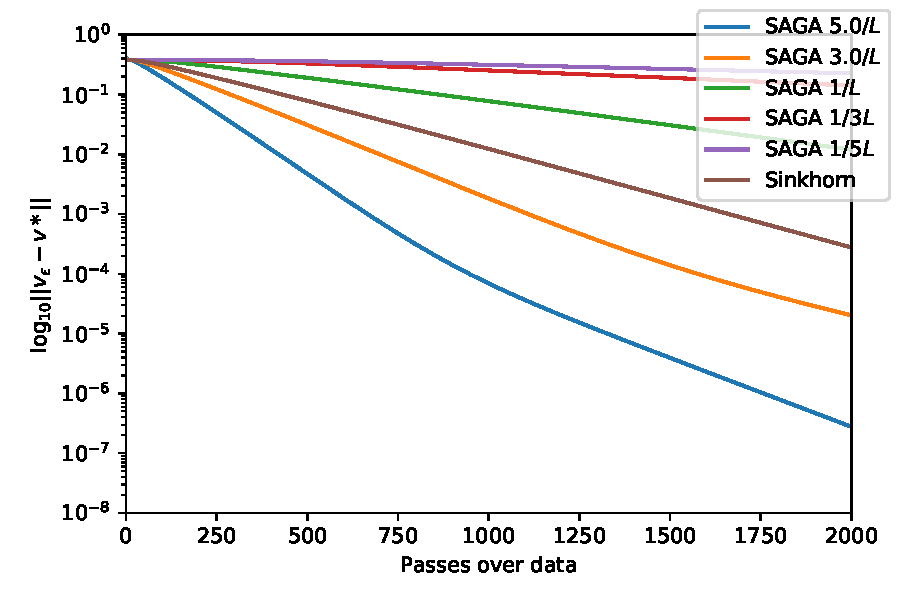
\includegraphics[width=0.49\linewidth]{figures/lr_bench_saga.pdf}
    \caption{Convergence of SAGA algorithm for different learning rates on two randomly generated histograms of size 500. 50 independent runs were averaged.}
\end{figure}

Observed convergence is linear after a certain number of passes over the data in those examples, which confirm the theoretical guarantees of the SAG and SAGA algorithm. 

As recommended in \cite{schmidt_minimizing_2013}, the three learning rates $1/L$, $3/L$ and $5/L$ are tested for the SAG algorithm. Depending on the chosen learning rate, improvement over Sinkhorn's algorithm can be obtained or not, which is a crucial information when trying to apply the algorithms on very large scale settings. Notably here, both $3/L$ and $5/L$ show very significant improvements over Sinkhorn.

For the SAGA algorithm, the theoretical convergence guarantee is proven for a learning rate of $1/3L$. We try this learning rate along with some others such as $1/5L$, $1/L$, $3/L$ and $5/L$. We note that, although no convergence guarantees exist for these values, SAGA algorithm has a behavior very similar to the SAG algorithm for the same pairs of learning rate ($1/nL$). This implies that SAGA doesn't show any significant advantage or disadvantage over SAG for this particular example. 

The optimal values all convergence rate are compared against were obtained by running Sinkhorn's algorithm up to convergence of the solution to machine precision.

We now study the properties of stochastic optimization on a real world dataset, for the task of image retrieval described in \cite{rubner_earth_2000}. For this, we work with the INRIA Holiday dataset \cite{forsyth_hamming_2008}\footnote{The dataset is available for download at \href{http://lear.inrialpes.fr/~jegou/data.php\#holidays}{\url{http://lear.inrialpes.fr/~jegou/data.php\#holidays}}.}. The pictures are preprocessed and converted from RGB to the CIE-Lab color space \cite{wyszecki_color_2000}, which was in turn uniformly quantized into $32^3$ bins in a 3D histogram. Since much of those bins are empty (the range of color of a dataset of natural images is limited and RGB doesn't capture all the color space available from the CIE-Lab color space), we prune the empty bins in the histograms and represent all images with histograms of size 4128. We note that by opposition to the last experiment, representation of the images in this form are typically very sparse. The cost function is the $L_2$ norm over the CIE-Lab color space.

With this representation, we compute 10 pairwise distances between images from the dataset selected at random and show the convergence results for SAG, SAGA and Sinkhorn. $\varepsilon$ was set to 0.01. We compare the results to an optimal dual variable $\bm{v}^*$ which corresponds to the best obtained dual variable across all methods.

\begin{figure}[h]
    \begin{subfigure}{.49\linewidth}
        \centering
        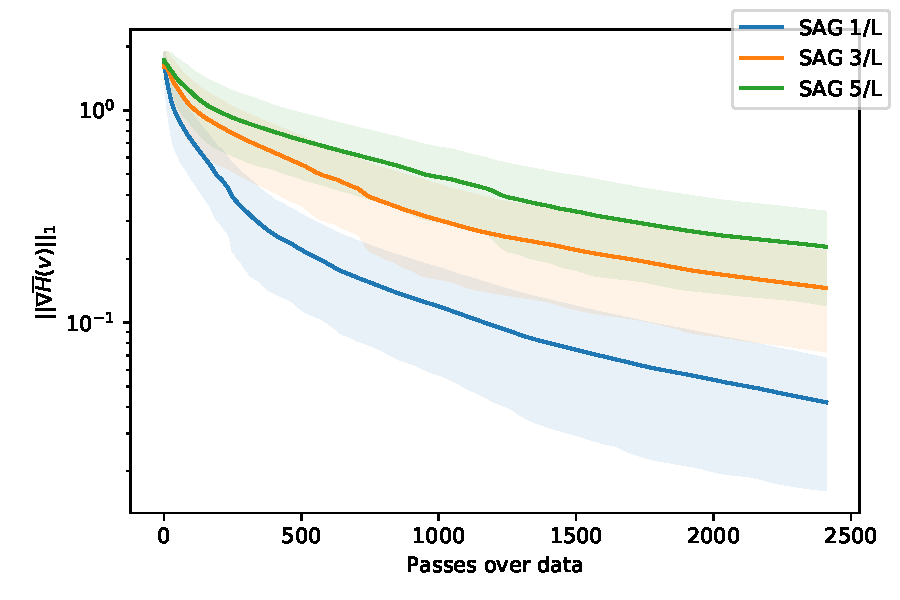
\includegraphics[width=\linewidth]{figures/sag_image_retreival_avg.pdf}
        \caption{Evolution of $||\nabla\overline{H}(v)||_1$.}
    \end{subfigure}
    \begin{subfigure}{.49\linewidth}
        \centering
        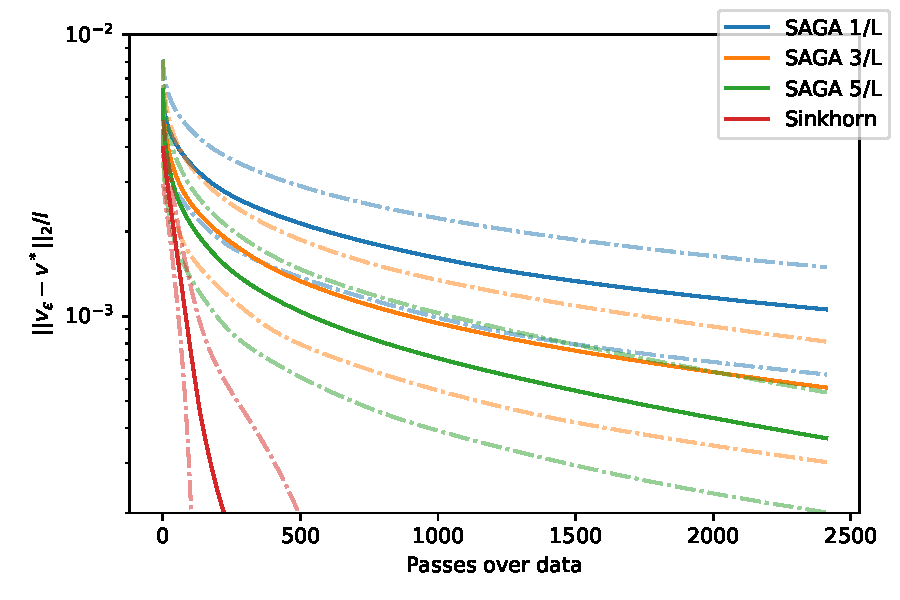
\includegraphics[width=\linewidth]{figures/sag_image_retreival_vs_avg.pdf}
        \caption{Convergence of SAG algorithm for different learning rates.}
    \end{subfigure}
    \caption{Convergence of SAG on 10 pairs of images. Dashed lines and filled areas represent deviation from the mean (solid line).}
\end{figure}

\begin{figure}[h]
    \begin{subfigure}{.49\linewidth}
        \centering
        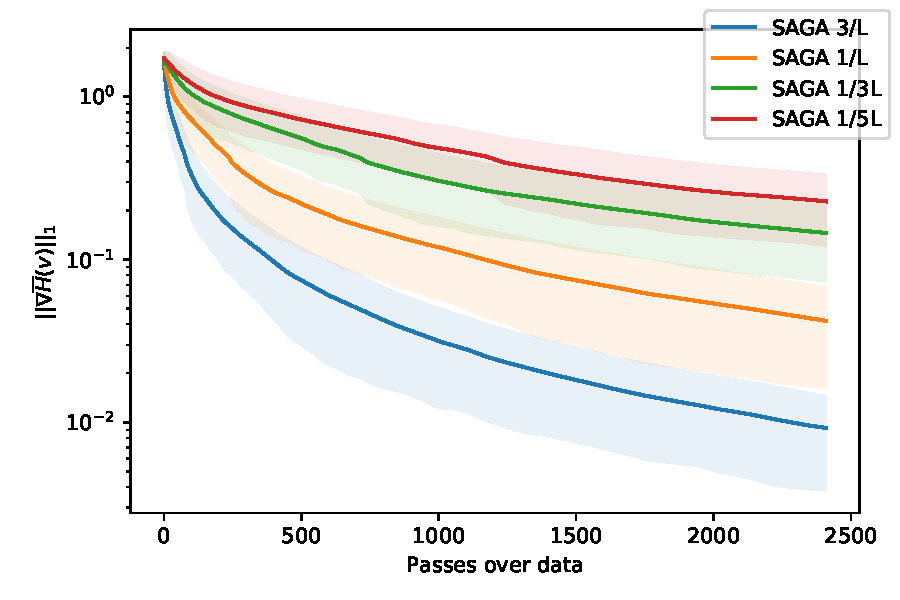
\includegraphics[width=\linewidth]{figures/saga_image_retreival_avg.pdf}
        \caption{Evolution of $||\nabla\overline{H}(v)||_1$.}
    \end{subfigure}
    \begin{subfigure}{.49\linewidth}
        \centering
        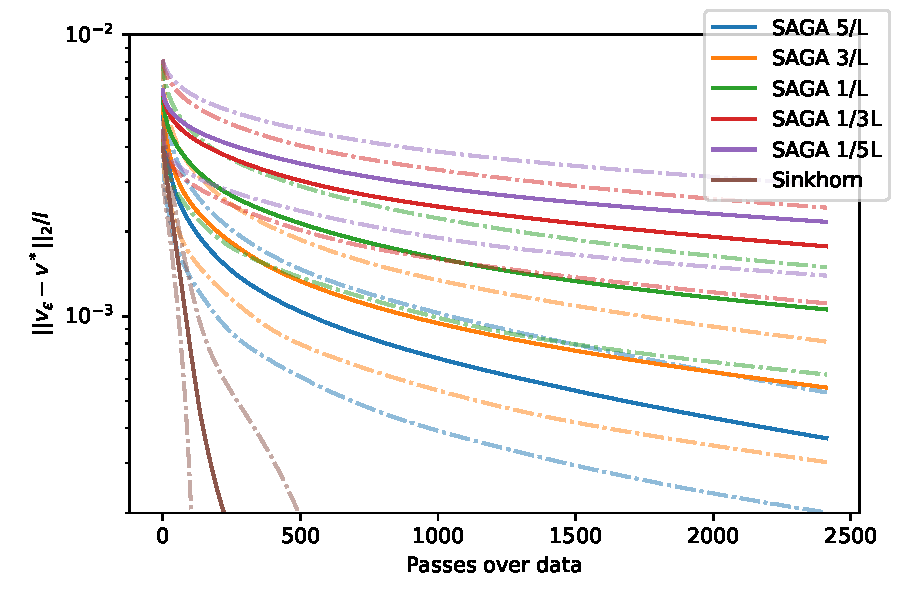
\includegraphics[width=\linewidth]{figures/saga_image_retreival_vs_avg.pdf}
        \caption{Convergence of SAG algorithm for different learning rates.}
    \end{subfigure}
    \caption{Convergence of SAGA on 10 pairs of images. Dashed lines and filled areas represent deviation from the mean (solid line).}
\end{figure}

In this example, Sinkhorn was consistently faster than the other optimization methods which had a convergence rate close to $O\left(\frac{1}{k}\right)$. For SAG and SAGA, the overall best performing learning rate was $5/L$ in terms of speed of convergence. It however gave some poor results for SAGA in some cases where the gradient did not converge to 0. 

\subsection{Semi-discrete Optimal Transport}
In semi-discrete optimal transport, $\mu$ can be an arbitrary measure and the other measure $\nu = \sum_{j=1}^J \mathbf{\nu}_j \delta_{y_j}$ is discrete \cite{peyre_computational_2018}. We therefore need to work with the expectation form of the dual and semi dual problem presented in \ref{section:stoch_formulation}. We recall here the semi-dual form of the problem \eqref{eq:stoch-semi-dual}: 
\begin{align*}
    W_\varepsilon(\mu, \nu) = \max_{v}\  \mathbb{E}_{X}[h_\varepsilon(X, v)]
\end{align*}
$X$ follows the law of $\mu$ in that case, and $h_\varepsilon$ has been defined above. The gradient aggregation algorithms such as SAG and SAGA cannot be applied as is to such problem, but the SG algorithms still fits to its constraints, since it only needs a random variable to sample from. 

A way to fall back to a setting were the gradient aggregation family of algorithms is applicable is to discretize the continuous measure and approximate it with a discrete one. This method has the drawback of making the obtained solution inexact due to discretization noise, and is therefore not studied in this report.

\subsubsection{Stochastic gradient algorithm for semi-discrete OT}

The SG algorithm applied to the semi-discrete setting is detailed in algorithm \ref{alg:sg_semi_discrete}. The convergence rate is guaranteed to be $O(1/\sqrt{k})$ by using averaging of the iterates $\bm{v}$ \cite{polyak_acceleration_1992} (line 5 in algorithm \ref{alg:sg_semi_discrete}) since the problem is not strongly convex.

\begin{figure}[h]
    \centering
    \begin{minipage}{.8\linewidth}
    \begin{algorithm}[H]
        \caption{SG algorithm for semi-discrete OT}\label{alg:sg_semi_discrete}
        \begin{algorithmic}[1]
            \State $\tilde{\bm{v}} \gets 0_J, \bm{v} \gets \tilde{\bm{v}}$
            \For {$k=1, ...,K$} 
                \State Sample $x_k$ realization of $X$ following $\mu$
                \State $\tilde{\bm{v}} \gets + \frac{\text{step}}{\sqrt{k}} \nabla_v \overline{h}_\varepsilon(x_k, \tilde{\bm{v}})$
                \State $\bm{v} \gets \frac{1}{k}\tilde{\bm{v}} + \frac{k-1}{k}\bm{v}$
            \EndFor
        \end{algorithmic}
    \end{algorithm}
\end{minipage}
\end{figure}

\subsubsection{Case study of semi-discrete OT for analysis of socio-economic data}

\paragraph{Problem formulation}\label{par:semi-discrete-prob}
We now study the properties of SGD algorithm applied to a semi-discrete OT problem based on real-world data. This experiment is inspired from Hartmann and Schuhmacher 's description of the delivery resource allocation problem \cite{hartmann_semi-discrete_2017} and Galichon's book on optimal transport for economics \cite{galichon_optimal_2018}. 

We will study here a problem of resource allocation based on open datasets available from the official French open dataset repository \href{www.data.gouv.fr}{\url{data.gouv.fr}}. Similarly to the delivery resource allocation problem studied in \cite{hartmann_semi-discrete_2017}, we consider a limited resource spatially scattered and a demand density across a territory. More specifically, we consider here a set of $J$ middle schools as the ressource (that is indeed spatially distributed), that we can assimilate to a discrete measure over a territory. That measure is supported by $\mathcal{Y} = \{1, .., J\}$.

To model demand, we use the population density $\mu$ (in the sense of number of people divided by the occupied area), with the assumption that demand for school is roughly proportional to the population density of the area. The support of this continuous measure is a delimited territory. To model the transportation cost of people going to a school, we use the square distance on the territory, or $L_2$ norm. For any inhabitant $x$ the cost to go to a school located at $y$ is therefore $\Phi(x, y) = |x-y|^2$. The support of $\mu$ is written $\mathcal{X}$.

Supply capacity for each school is represented by the the total number of students at the school. The total school supply sums to one which equates the total demand. 

A rudimentary way of solving this ressource allocation problem would be to only take into account the supply and demand without modelling any form of side-effect of high demand (such as high price, or in our case, the high entry level of the school). Everybody would then choose the school such as to maximize a \emph{utility} function $u(x) = \max_{j\in\{1, ..., J\}} {-\Phi(x, y)}$. 
The set of people preferring school $j$ over other schools is
\begin{align*}
    \mathcal{X}_j^0 \triangleq \{ x \in \mathcal{X} \ |\ \Phi(x, y_j)\leq \Phi(x, y_k), \forall k\}
\end{align*}
This corresponds to a Voronoi tessellation of the territory with the schools being the centers of the Voronoi cells.
Demand for school $j$ is $\mathbb{P}(x\in \mathcal{X}_j) = \int_{\mathcal{X}_j} \text{d}\mu(x)$. 

Now, if we consider that school have an entry level $\mathbf{p} = (\mathbf{p}_j)_{j\in\{1, ..., M\}}$ that changes with demand, and we assume that utility is written\footnote{This modelling could obviously be discussed, since the assumption that people will preferably choose a school with low entry level and closer to them is debatable. The assumption is made here to show a possible way of posing the problem in terms of optimal transport.} 
\begin{align*}
    u(x) = \max_{j\in\{1, ..., J\}} {-\mathbf{p}_j - \Phi(x, y_j)}
\end{align*}
We write $q_j$ the demand for school $j$. At market equilibrium, demand for a school equates the supply it provides and all schools are at complete capacity, hence $\mathbb{P}(x\in \mathcal{X}_j) = q_j$, with $\sum_j q_j = 1$.

\paragraph{A transportation problem}
A planner seeks to find an optimal assignment $\pi$ that minimizes the total transportation cost, while matching the population density with the corresponding schools. She would have
\begin{align*}
    \min_{\pi\in \Pi(\mu, q)} \int_{\mathcal{X}, \mathcal{Y}} c(x, y)\text{d} \pi(x, y)
\end{align*}
This is the exact formulation of a semi-discrete transport problem with continuous measure $\mu$ and discrete measure $q = \sum_j \delta_{y_j} q_j$.

We now write the semi-dual form of the entropic regularization of the problem
\begin{align*}
    W_\varepsilon(\mu, q) = \max_{v\in\mathbb{R}^J} \mathbb{E}_X[\overline{h}_\varepsilon(X, \bm{v})]
\end{align*}
We recall the expression of $\overline{h}_\varepsilon$ and give some details about it in the setting of the case study. 
\begin{align*}
    \overline{h}_\varepsilon(x, \bm{v}) = \sum_{j=1}^J \bm{v}_j \bm{\nu}_j + 
    \begin{cases}
        -\varepsilon\log\left( \sum_{j=1}^J \exp\left(\frac{\bm{v}_j - c(x, y_j)}{\varepsilon}\right)\bm{\nu}_j \right) - \varepsilon & \text{if }\varepsilon > 0,\\
        \min_j (c(x, y_j) - \bm{v}_j) & \text{if }\varepsilon = 0
    \end{cases}
\end{align*}

Note also that the solution to the optimization problem is a smooth version of the Laguerre cells $\mathbb{L}_{\bm{v}}(y_j) \triangleq \left\{ x\in\mathcal{X}\ | \ c(x,y_j) - v_j \leq c(x, y_k) - v_k, \forall k \right\}$. It seems now that the semi-dual problem can be interpreted in terms of choosing a entry level $\mathbf{p}$ for all schools, by identifying $\mathbf{p}$ with $-\bm{v}$. $\overline{h}_\varepsilon$ then becomes 
\begin{align*}
    \overline{h}_\varepsilon(x, \mathbf{p}) = -\sum_{j=1}^J \mathbf{p}_j q_j + 
    \begin{cases}
        -\varepsilon\log\left( \sum_{j=1}^J \exp\left(\frac{-\mathbf{p}_j - c(x, y_j)}{\varepsilon}\right)q_j \right) - \varepsilon & \text{if }\varepsilon > 0,\\
        \min_j (c(x, y_j) + \mathbf{p}_j) & \text{if }\varepsilon = 0
    \end{cases}
\end{align*}
The problem therefore amounts to finding the price that maximizes the expected utility $u(x) = \min_{j\in\{1, ..., J\}} {\mathbf{p}_j + \Phi(x, y_j)}$ (and smoothed utility) of everyone while minimizing the global output of all schools (demand times the level of each school).

Possible applications of this kind of model range from defining the spatial assignment of public schools to identifying the weak points in the geographical repartition of schools and managing the attractiveness of all schools. 

\paragraph{Numerical experiments}

We implement the SG algorithm to solve the semi-discrete OT problem for the two measures represented on Figure \ref{fig:loire}. We use the squared distance as our cost function. This is based on the assumption that straight line distance is a good proxy for the travel distance, which might not be very accurate when there is a body of water between two points for example. A better distance function would use isochrone curves, but we assume that the straight line distance is a good enough approximation for this example. 

\begin{figure}[h]
    \centering
    \begin{subfigure}{.49\linewidth}
        \centering
        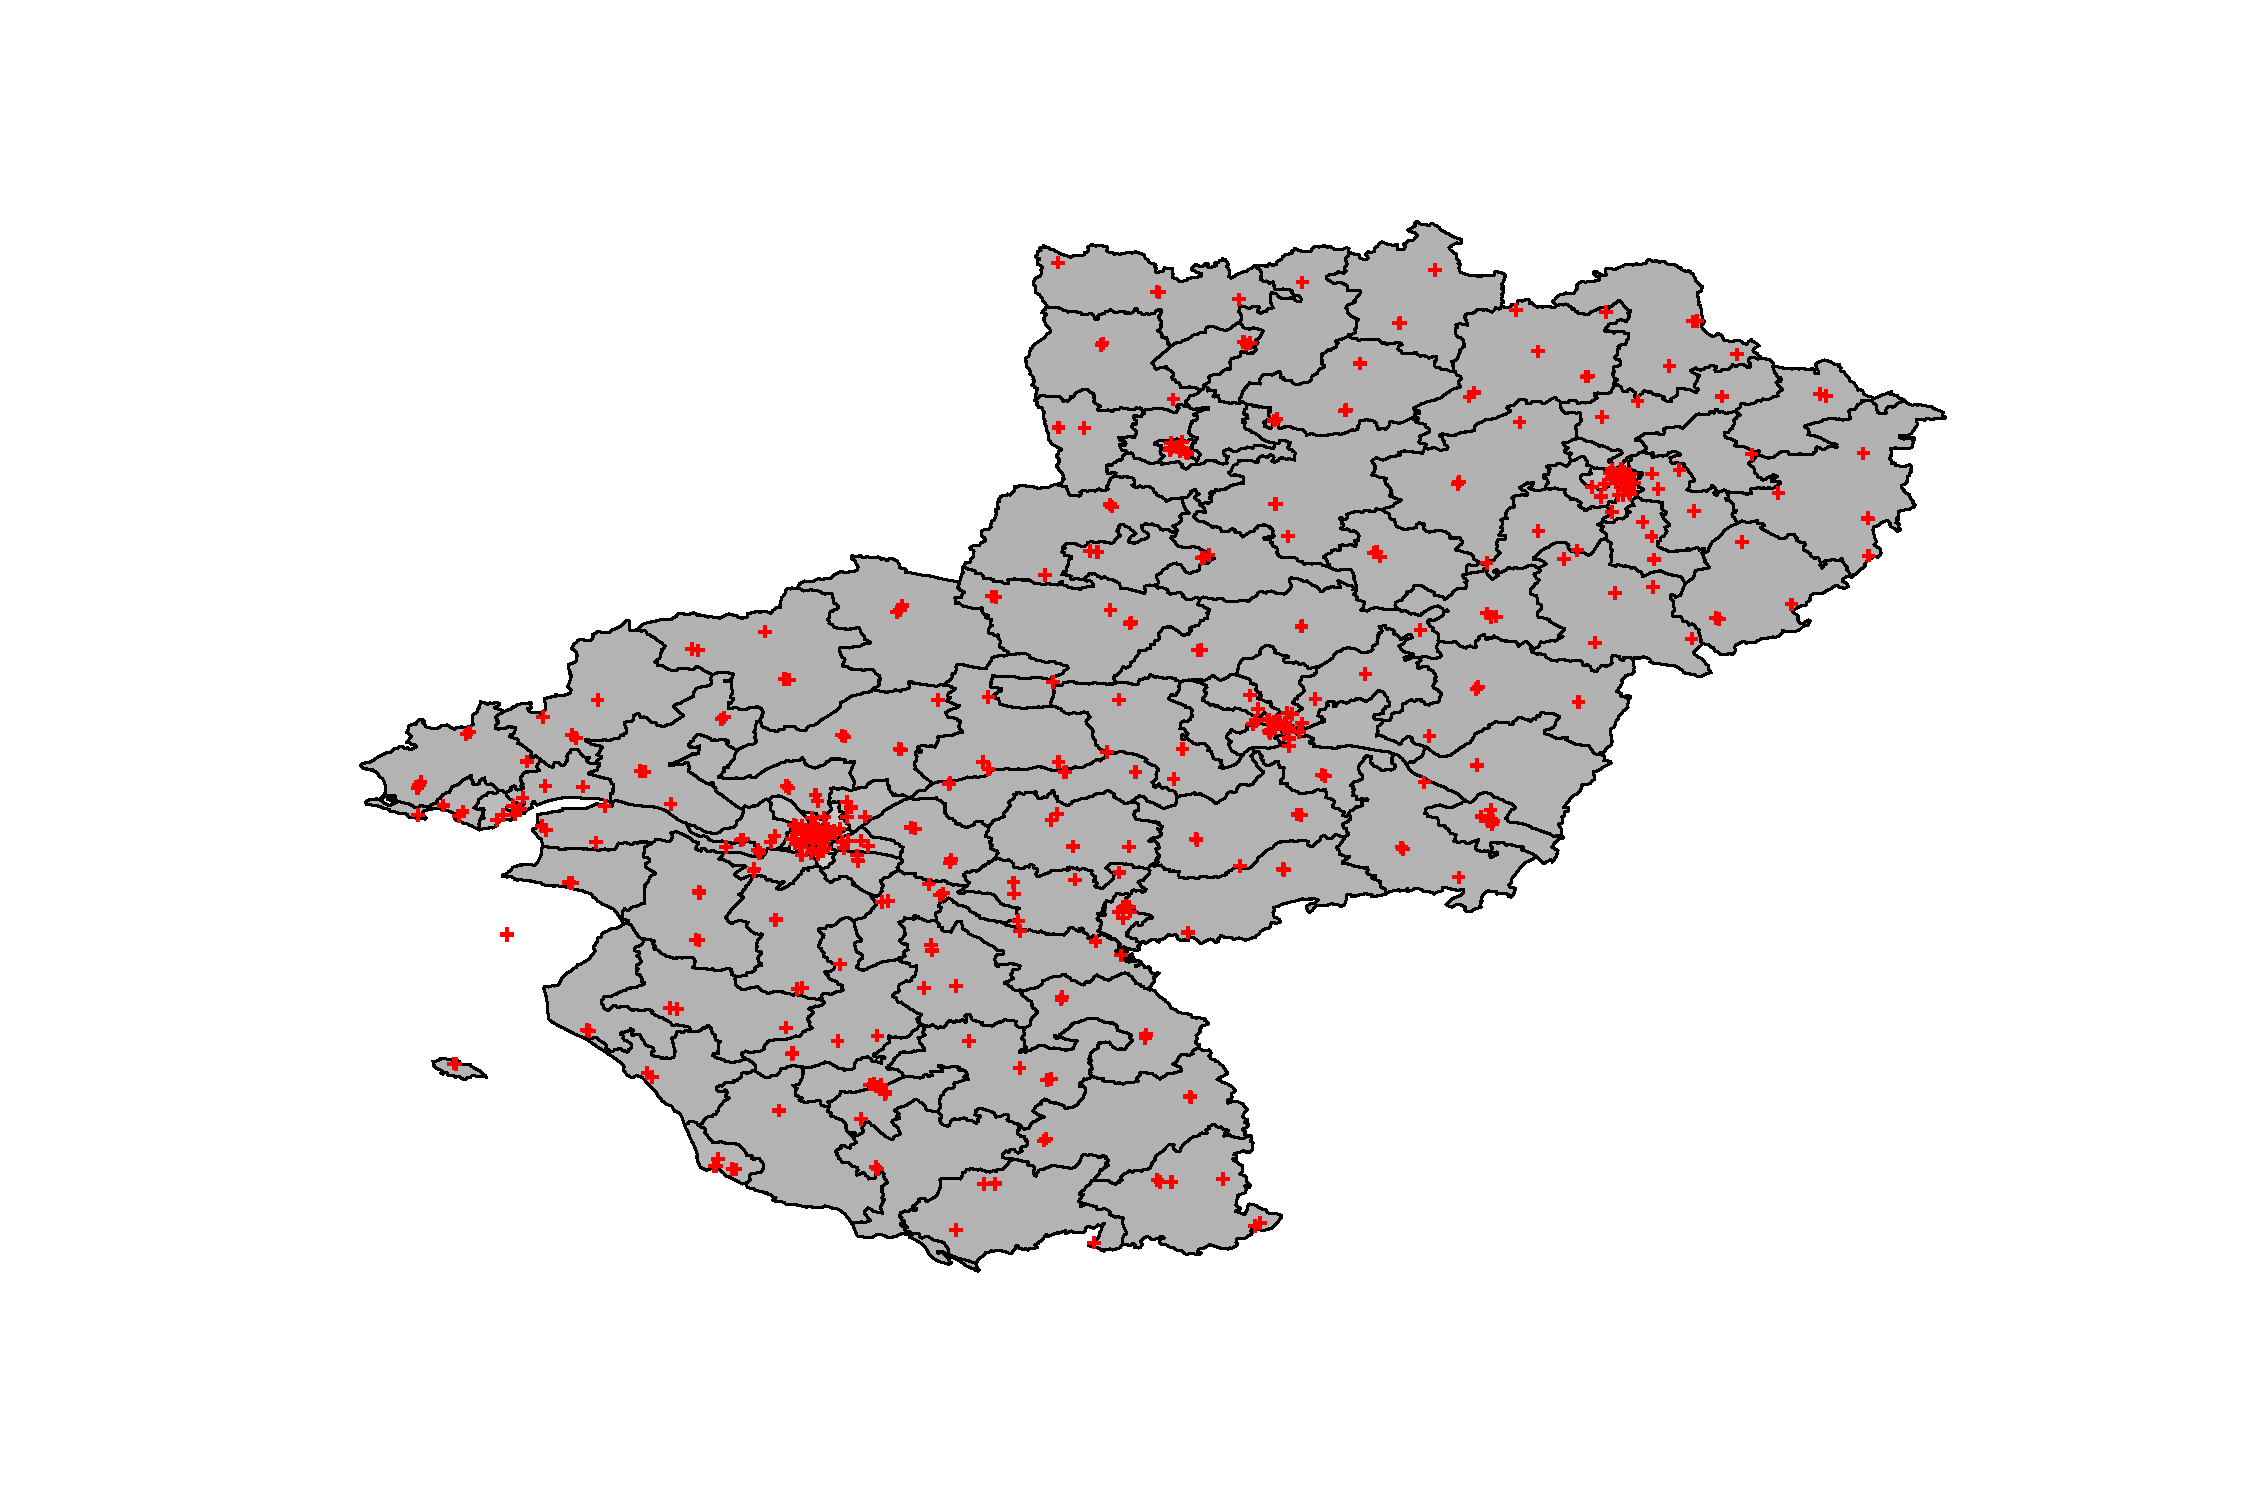
\includegraphics[width=\linewidth]{figures/nantes.pdf}
        \caption{School locations}
    \end{subfigure}
    \begin{subfigure}{.49\linewidth}
        \centering
        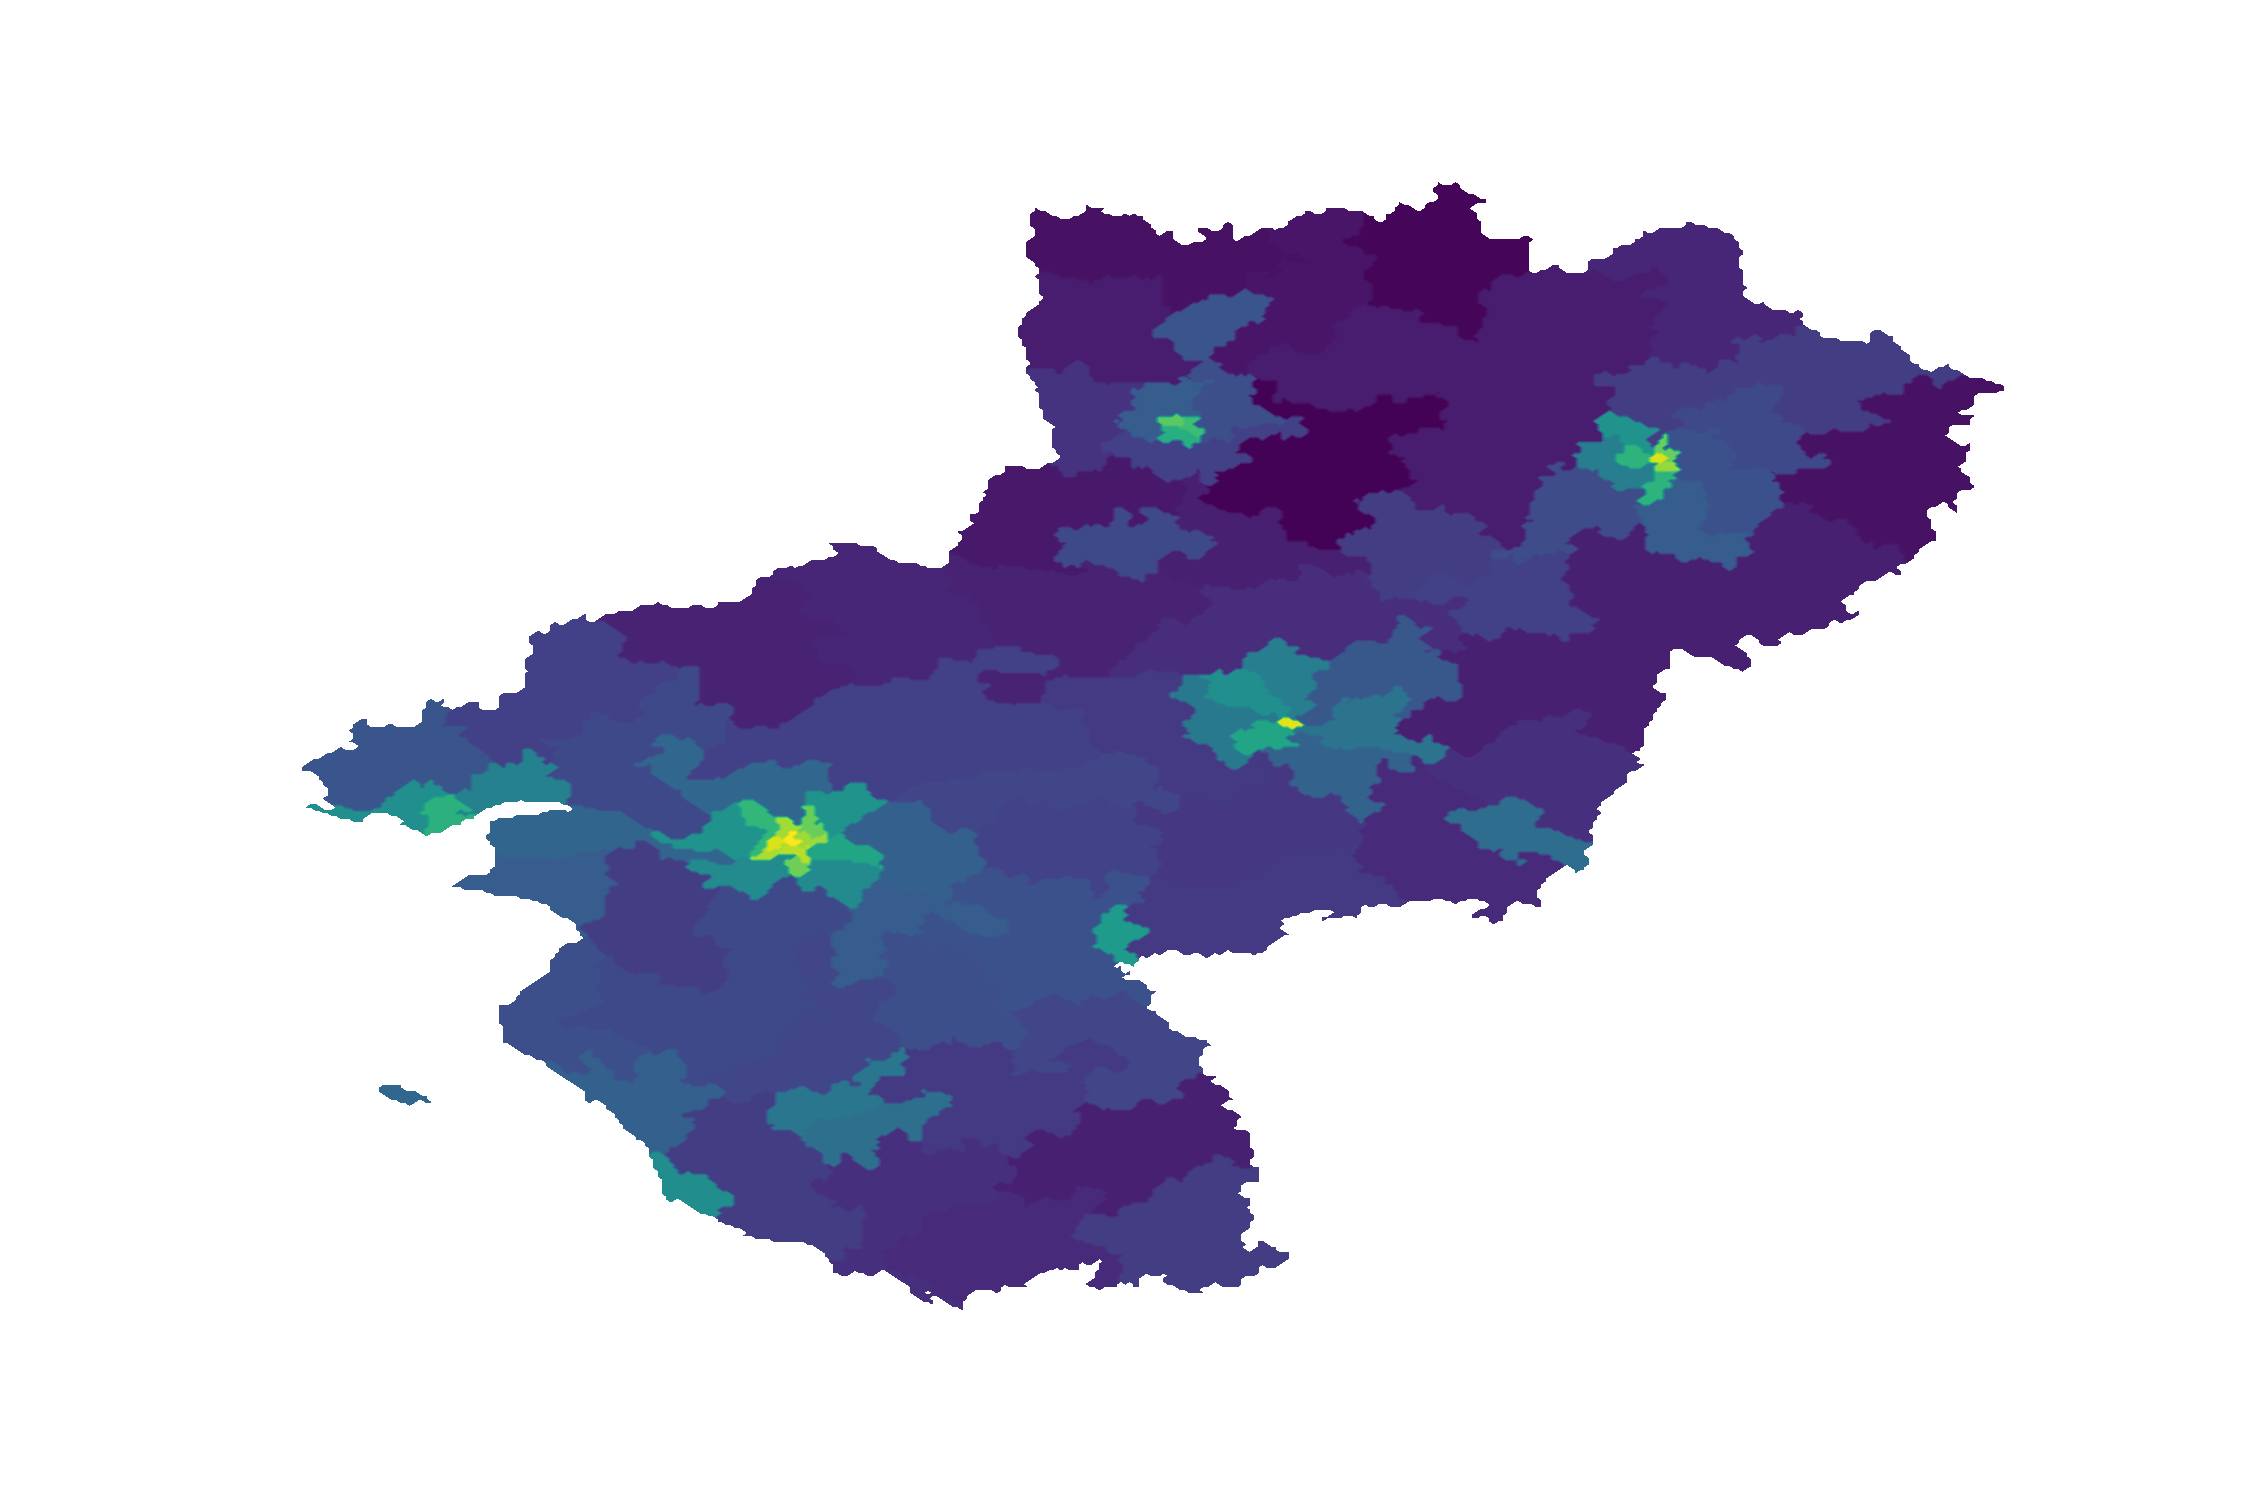
\includegraphics[width=\linewidth]{figures/nantes_log_density.pdf}
        \caption{Population log-density by ``cantons''}
    \end{subfigure}
    \caption{Example initial setting of the problem described in paragraph \ref{par:semi-discrete-prob} for the French administrative region ``Pays de la Loire''}
    \label{fig:loire}
\end{figure}

Setting the vector $\bm{v}$ to 0 would yield an assignment that coincides with the smoothed Voronoi tessellation of the territory. The smoothed $\overline{c}$-transform of $\bm{v}$ represents the expected utility at position $x$. The optimal function, computed after $10^8$ iterations of SG, is represented on Figure \ref{fig:loire-c-trans}. The Laguerre cells corresponding to the computed dual potential $\bm{v}$ are displayed on Figure \ref{fig:loire-cells}.

\begin{figure}[h]
    \centering
    \begin{subfigure}{.49\linewidth}
        \centering
        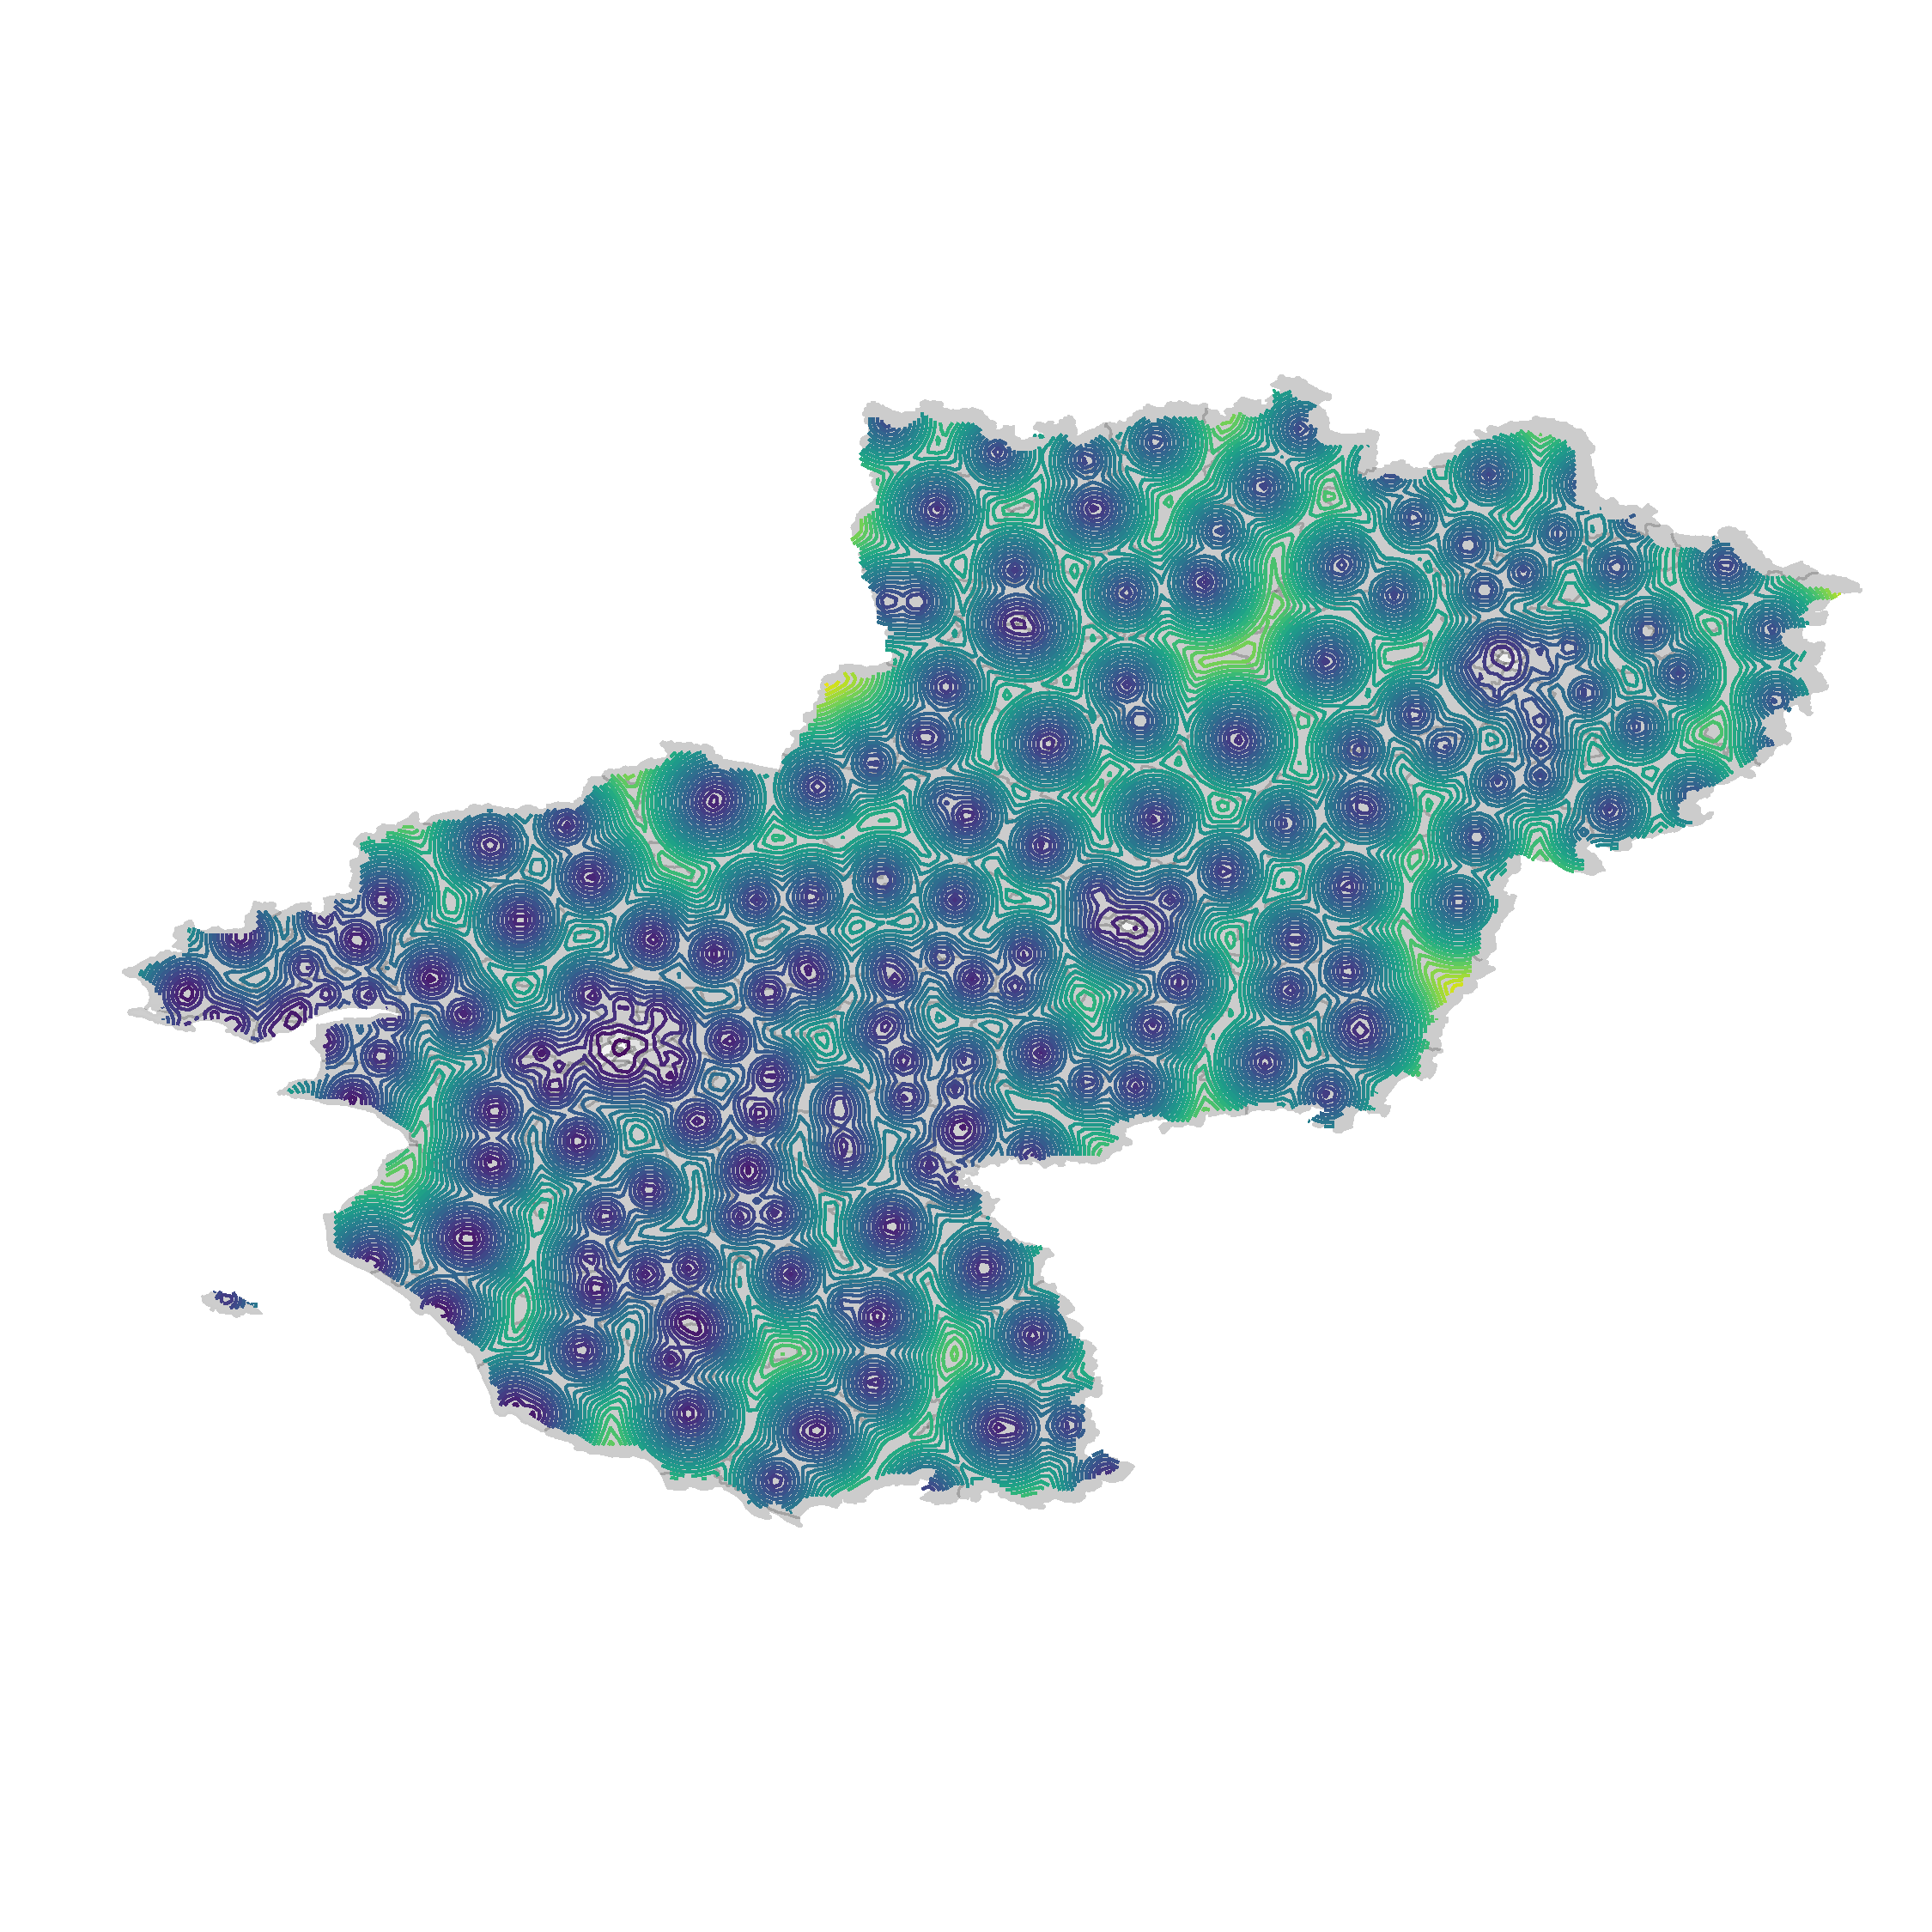
\includegraphics[width=\linewidth]{figures/opti_nantes.pdf}
        \caption{Smoothed $\overline{c}$-transform of an optimal $\bm{v}$, $\bm{v}^{\overline{c}, \varepsilon}$ for $\varepsilon = 0.01$.}
        \label{fig:loire-c-trans}
    \end{subfigure}
    \begin{subfigure}{.49\linewidth}
        \centering
        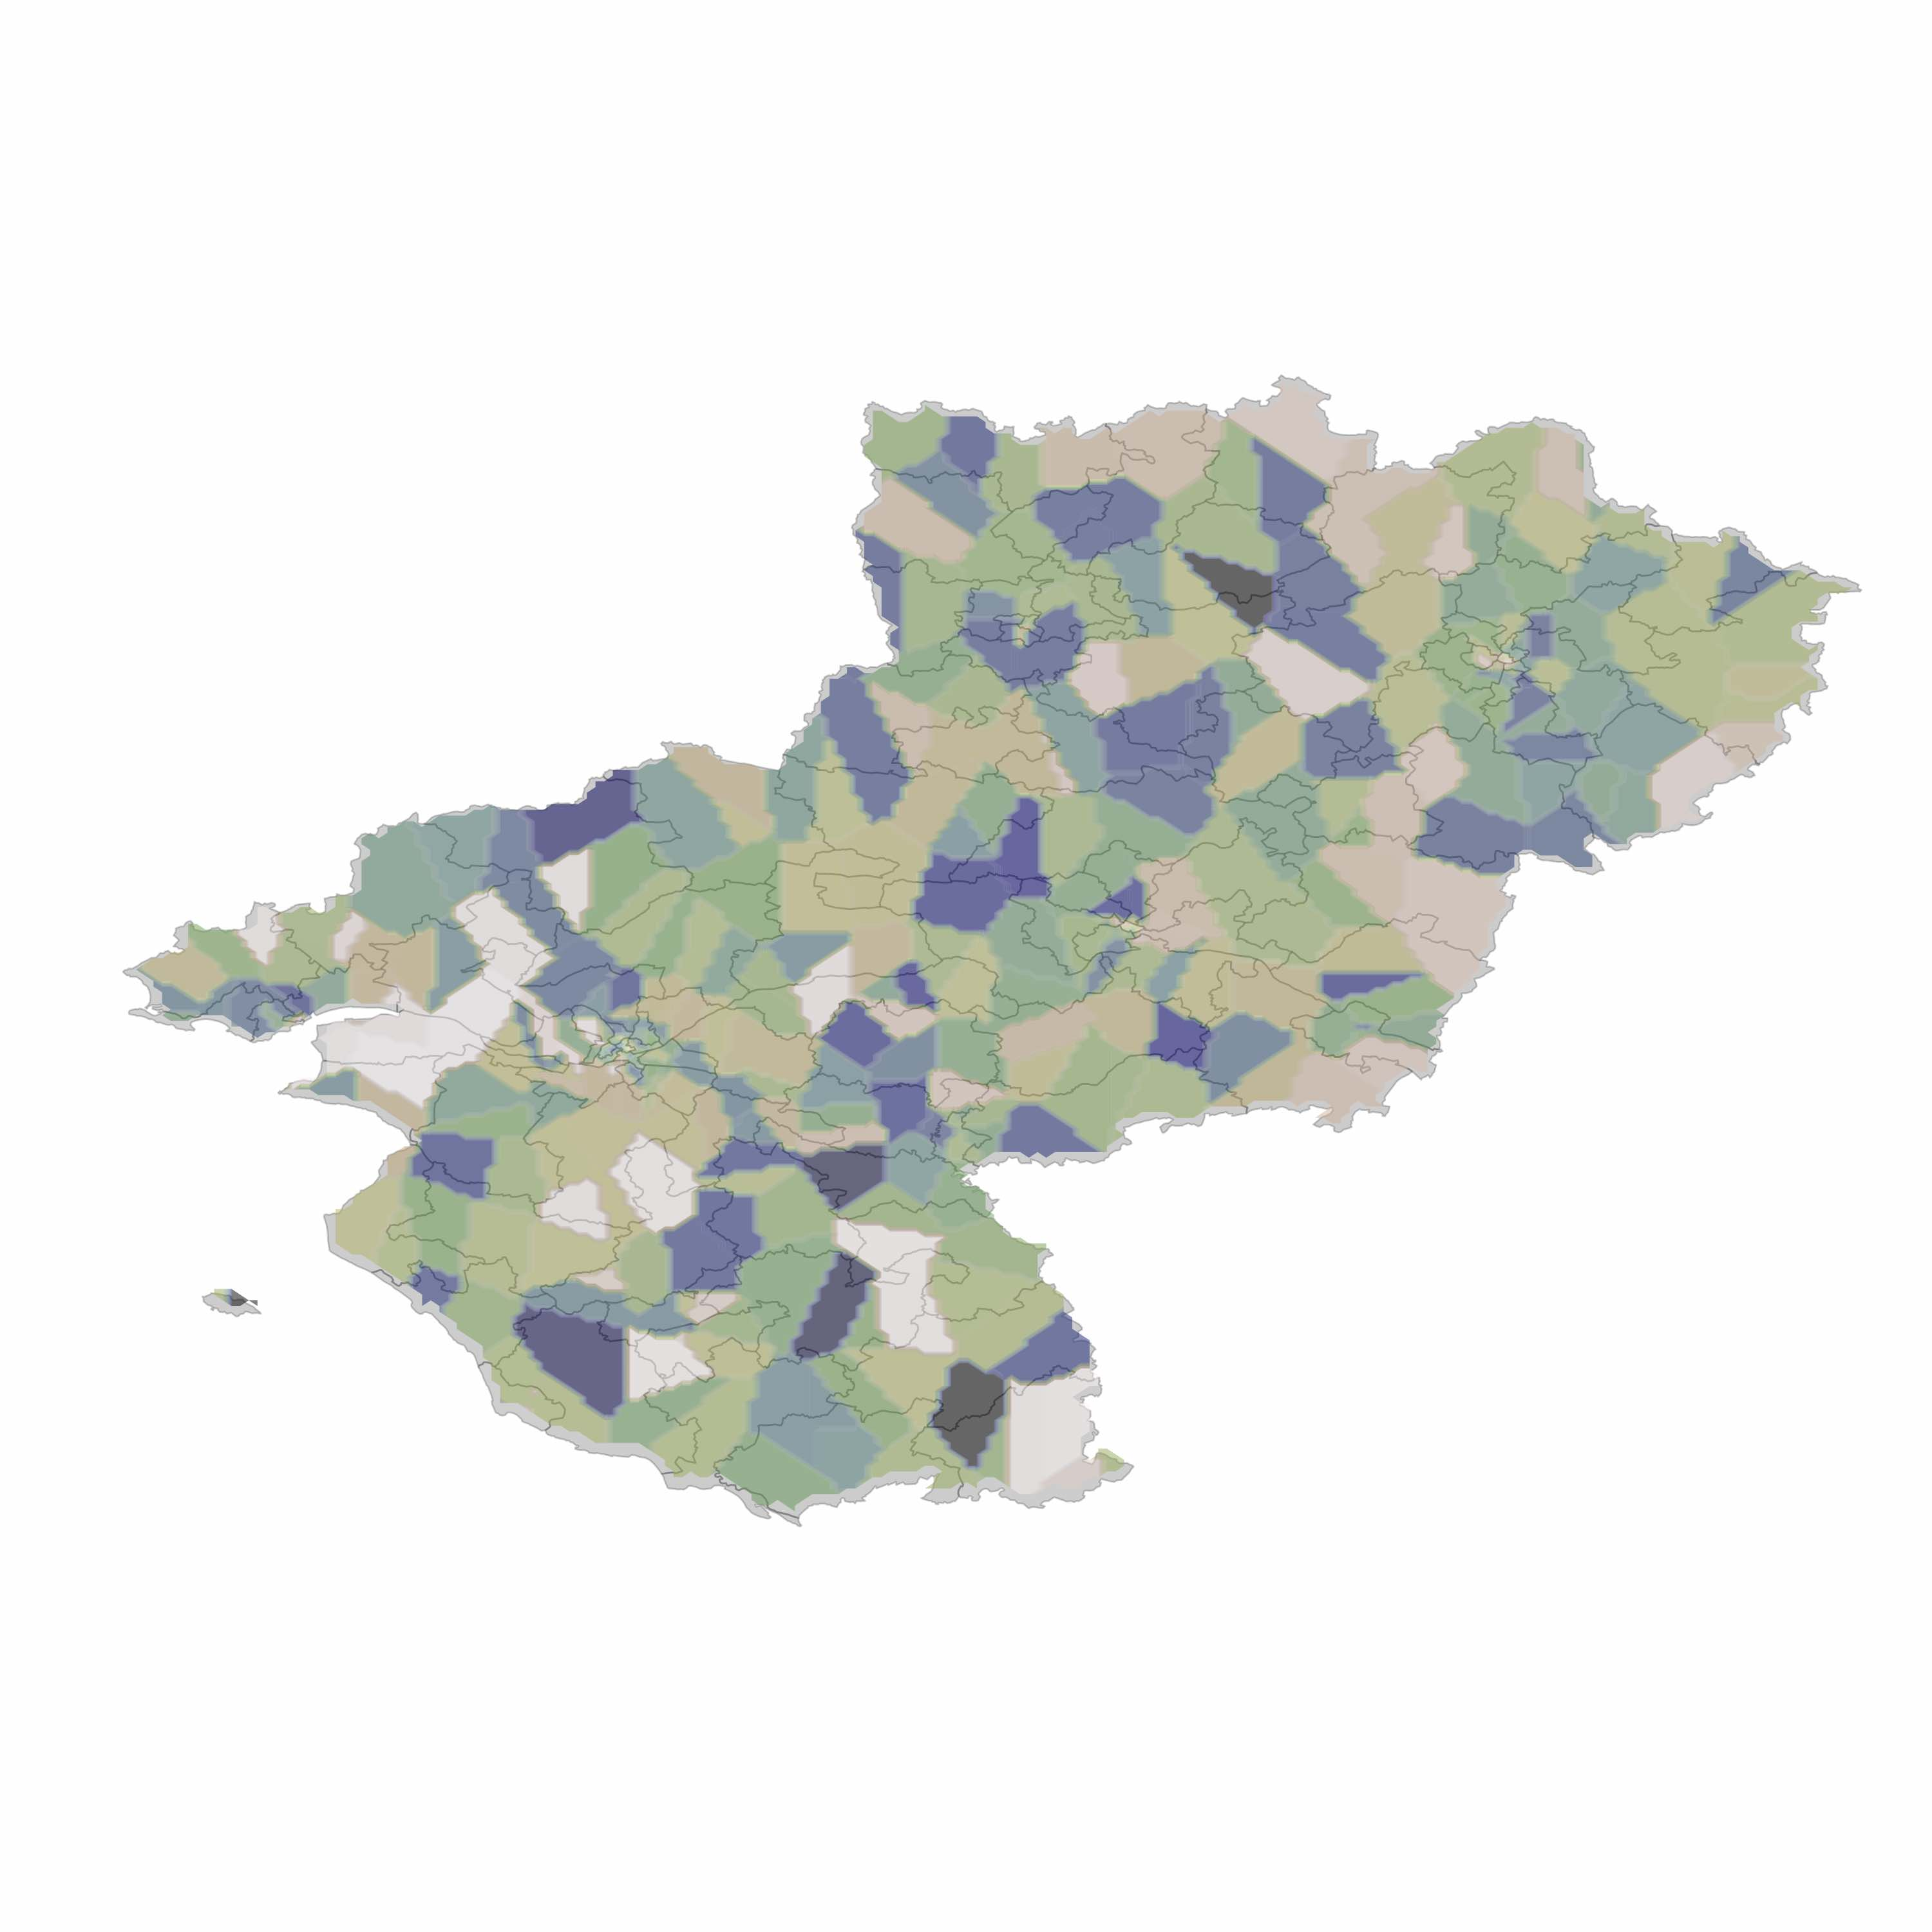
\includegraphics[width=\linewidth]{figures/opti_nantes_cells.jpg}
        \caption{Laguerre cells for the computed value of $\bm{v}$, corresponding to the assigned schools that minimizes the overall transportation cost with $\varepsilon = 0.01$.}
        \label{fig:loire-cells}
    \end{subfigure}
    \caption{Results for the problem illustrated on Figure \ref{fig:loire}}
\end{figure}


\begin{figure}[h]
    \centering
    \begin{subfigure}{.49\linewidth}
        \centering
        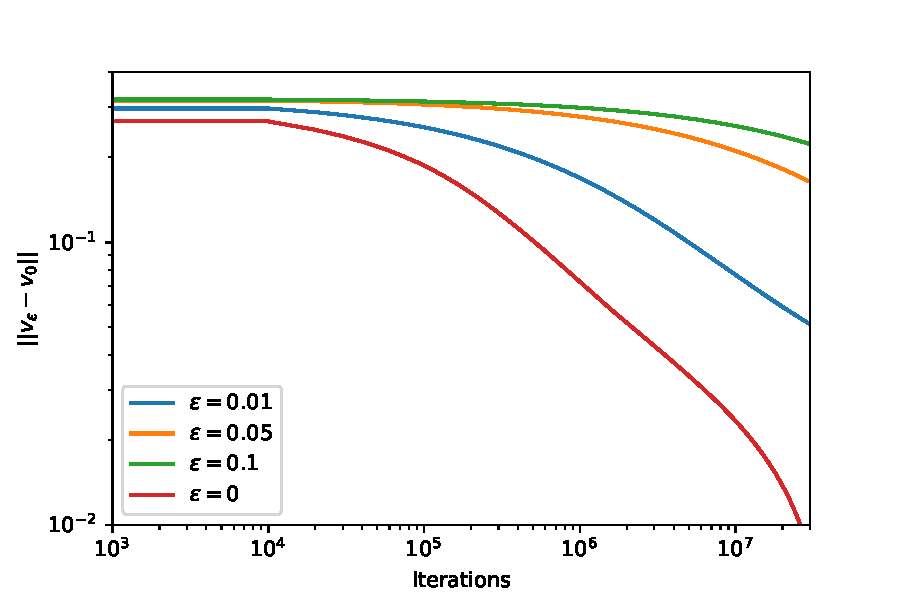
\includegraphics[width=\linewidth]{figures/semi_discrete_eps.pdf}
        \caption{Convergence towards unregularized solution.}
        \label{fig:eps-conv-semi-dis}
    \end{subfigure}
    \begin{subfigure}{.49\linewidth}
        \centering
        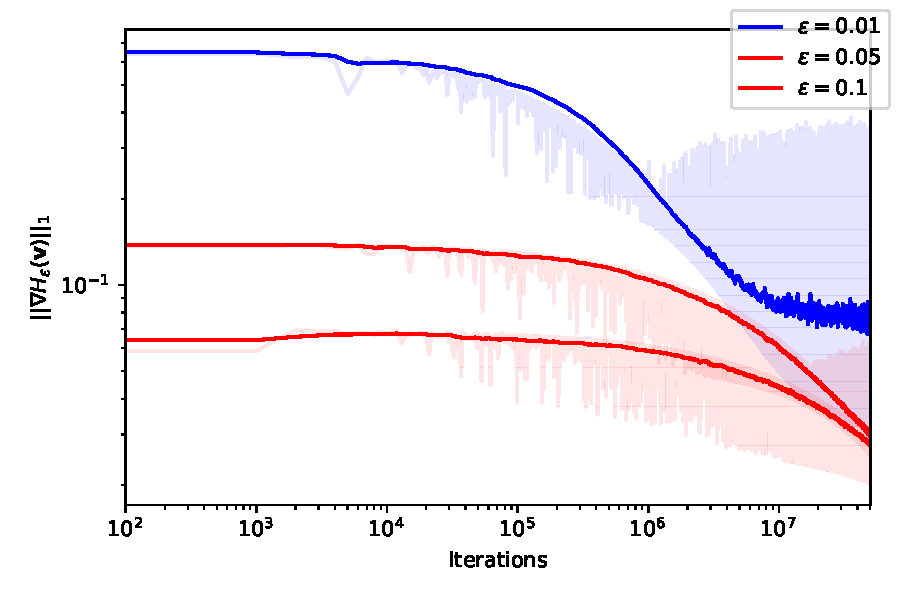
\includegraphics[width=\linewidth]{figures/grad_semi_discrete.pdf}
        \caption{Evolution of gradient of objective function.}
        \label{fig:eps-grad-semi-dis}
    \end{subfigure}
    \caption{Convergence of SG in the semi-discrete setting for different values of $\varepsilon$}
\end{figure}

Figure \ref{fig:eps-conv-semi-dis} shows the convergence plot for several values of $\varepsilon$ of the SG algorithm on the example displayed Figure \ref{fig:loire}. Figure \ref{fig:eps-grad-semi-dis} shows a moving average of the gradients during processing, lighter lines represent the real values.
Convergence is observed to be much slower than for the discrete setting with gradient aggregation algorithms, which is in accordance with theory. 

The iterates were compared against an optimal $\bm{v}_0^*$ obtained by running SG on the unregularized problem for $5\times 10^8$ iterations (5 times more than plotted).
Note that for $\varepsilon \neq 0$, the iterates are not expected to converge to the unregularized solution and will rather converge to some other value.

\begin{figure}[h]
    \centering
    \begin{subfigure}{.35\linewidth}
        \centering
        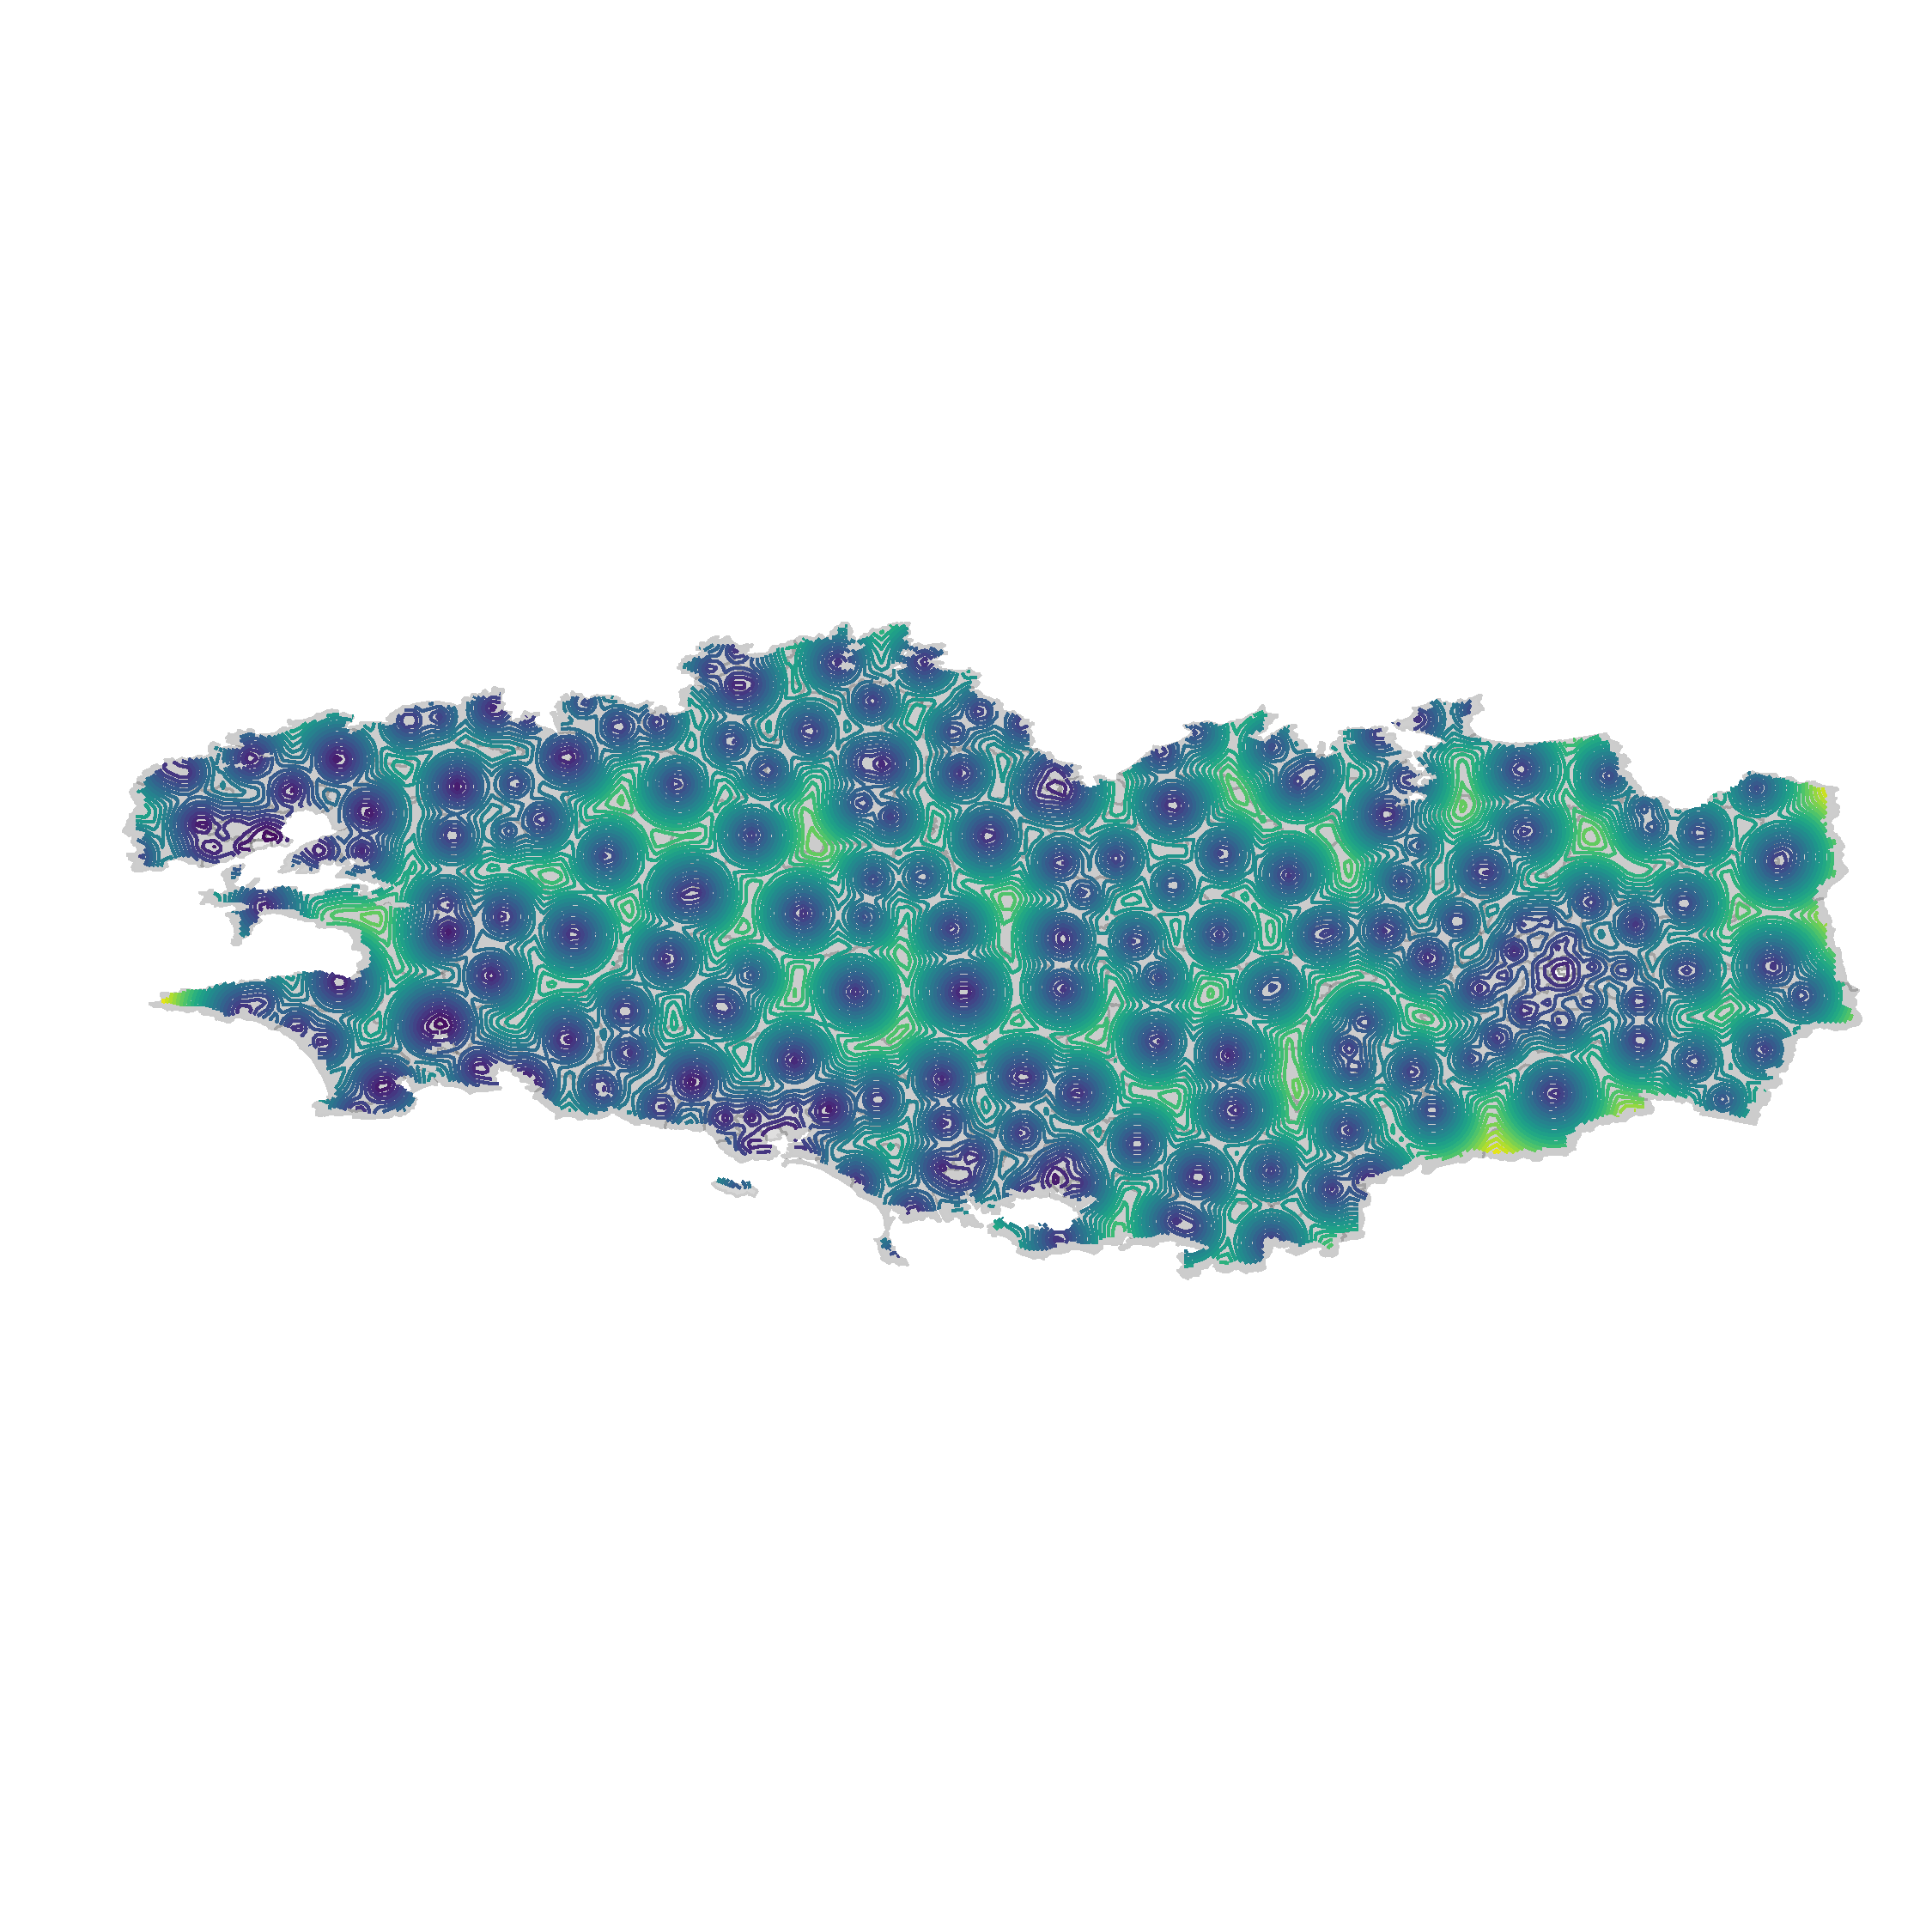
\includegraphics[width=\linewidth]{figures/opti_rennes.pdf}
        \caption{Smoothed $\overline{c}$-transform of an optimal $\bm{v}$, $\bm{v}^{\overline{c}, \varepsilon}$ for $\varepsilon = 0.01$.}
    \end{subfigure}
    \begin{subfigure}{.35\linewidth}
        \centering
        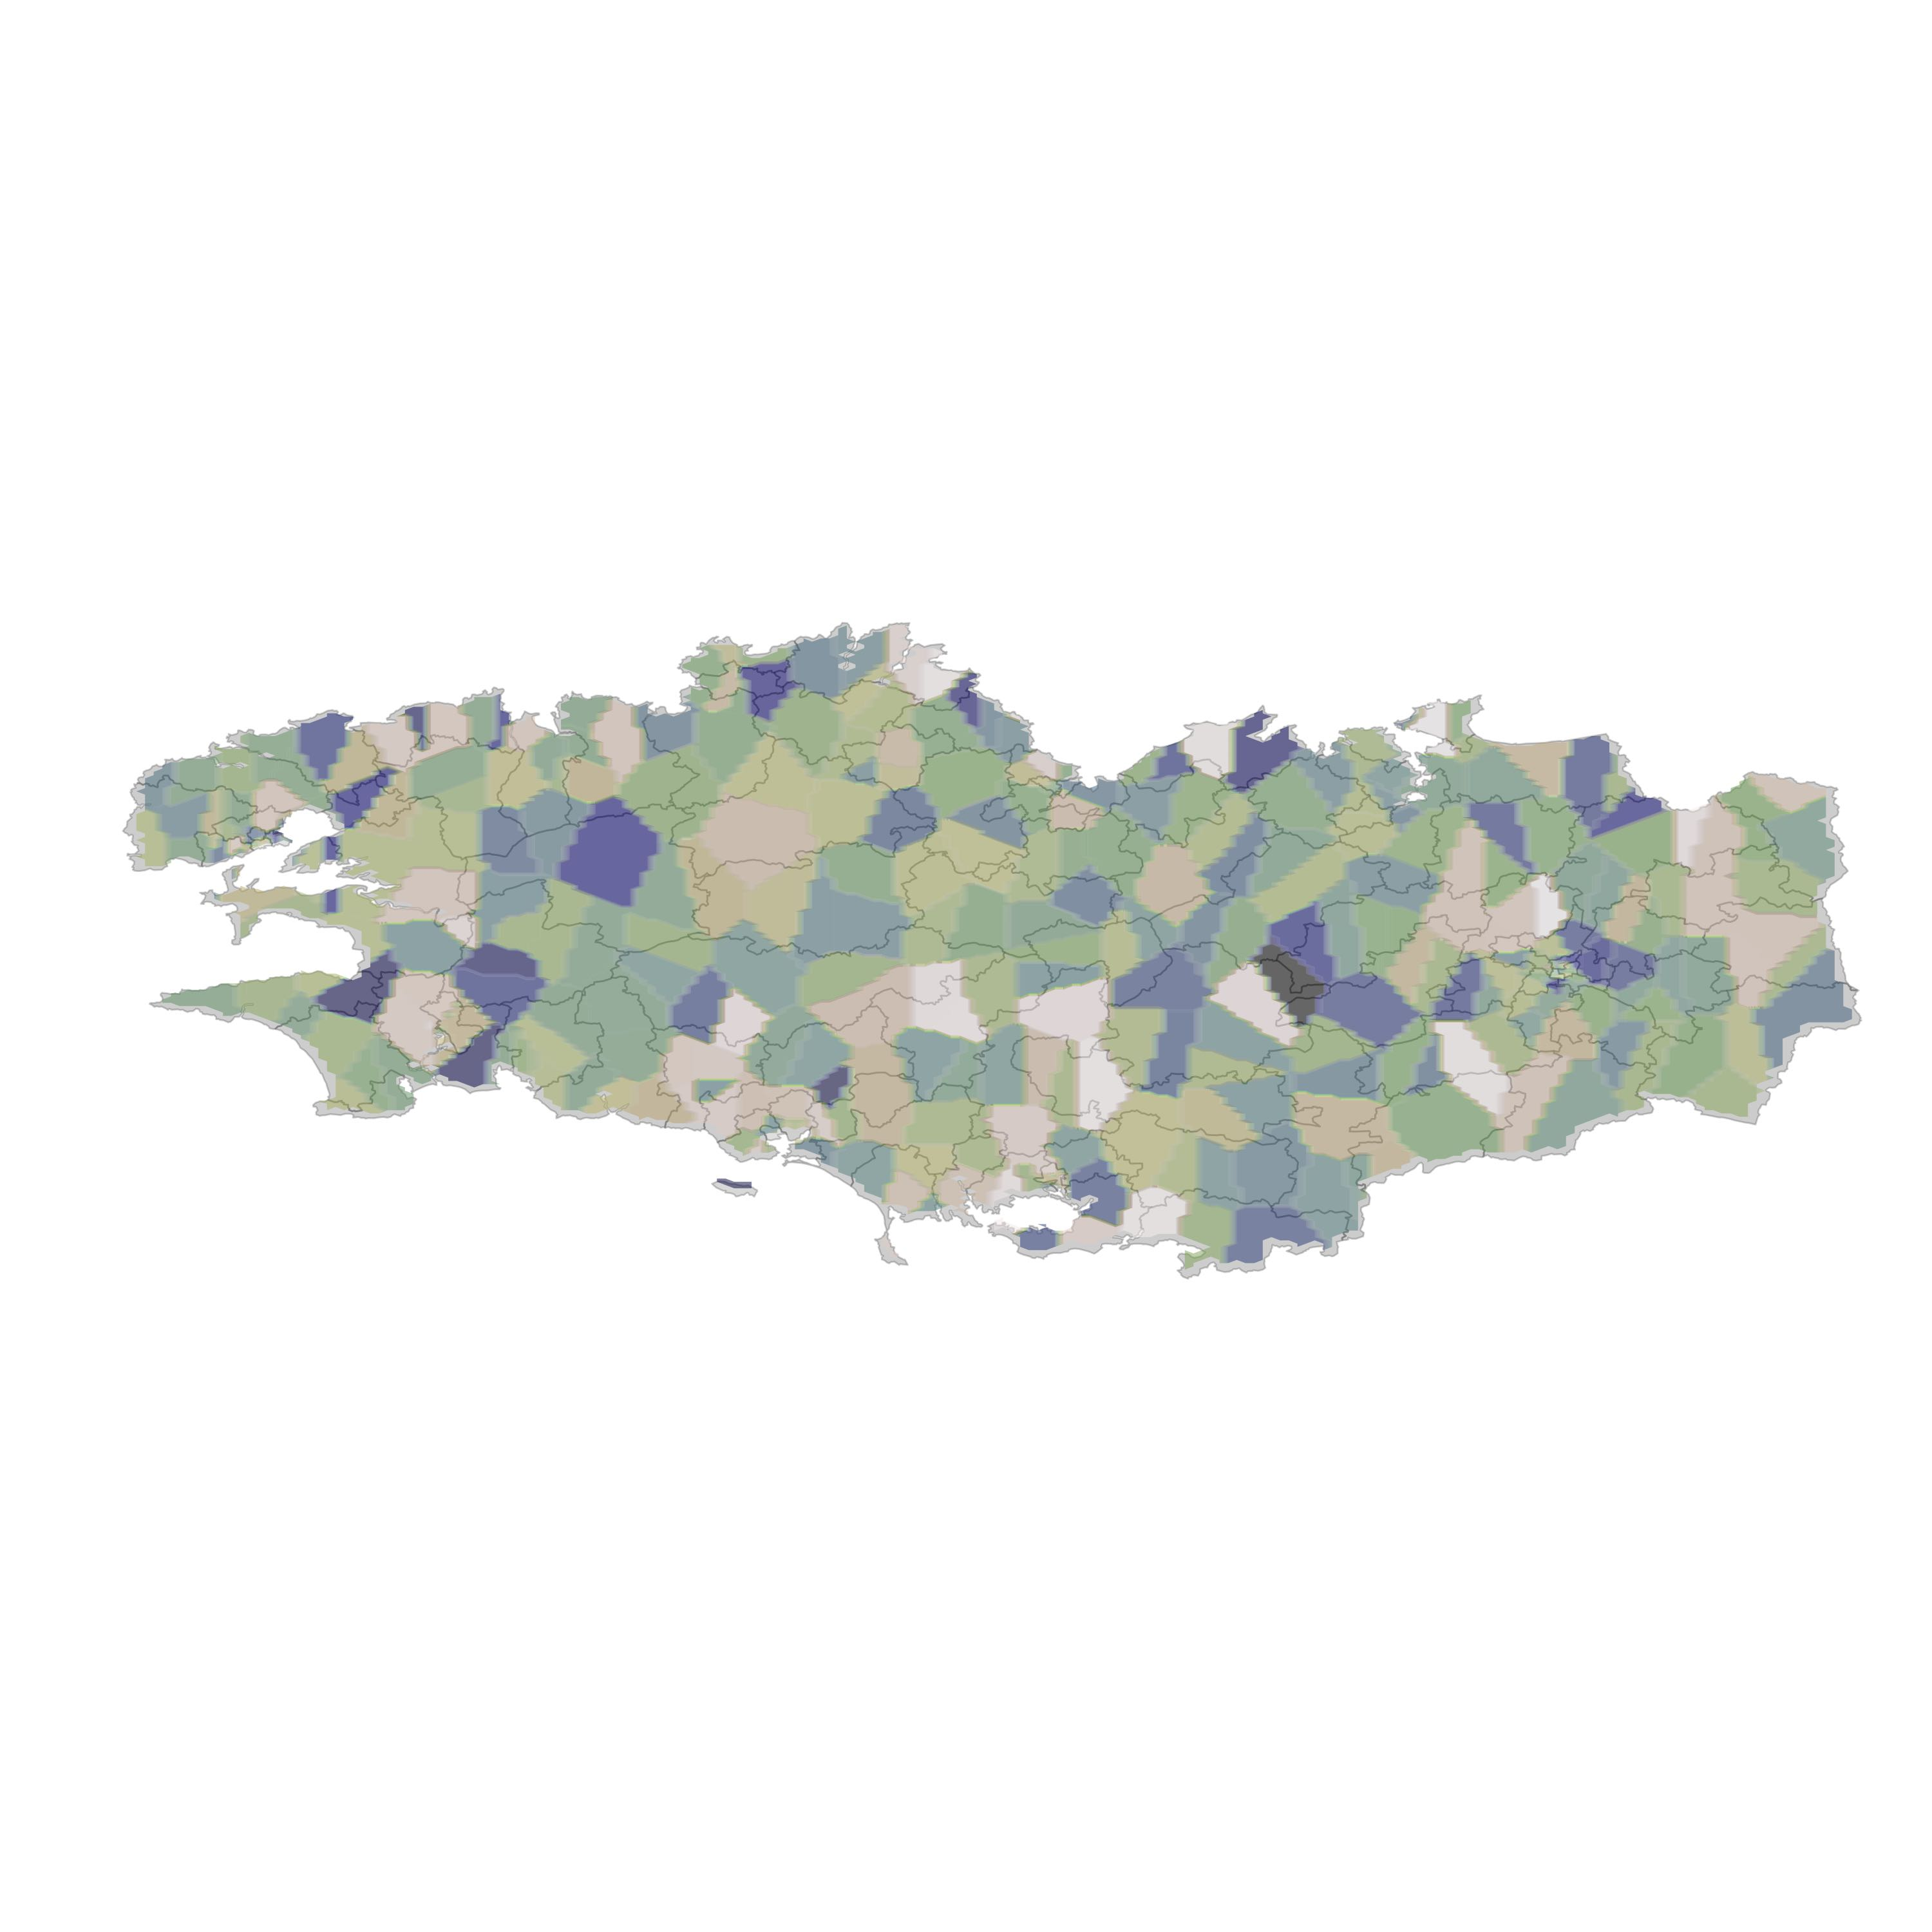
\includegraphics[width=\linewidth]{figures/opti_rennes_cells.jpg}
        \caption{Laguerre cells.}
    \end{subfigure}
    \begin{subfigure}{.49\linewidth}
        \centering
        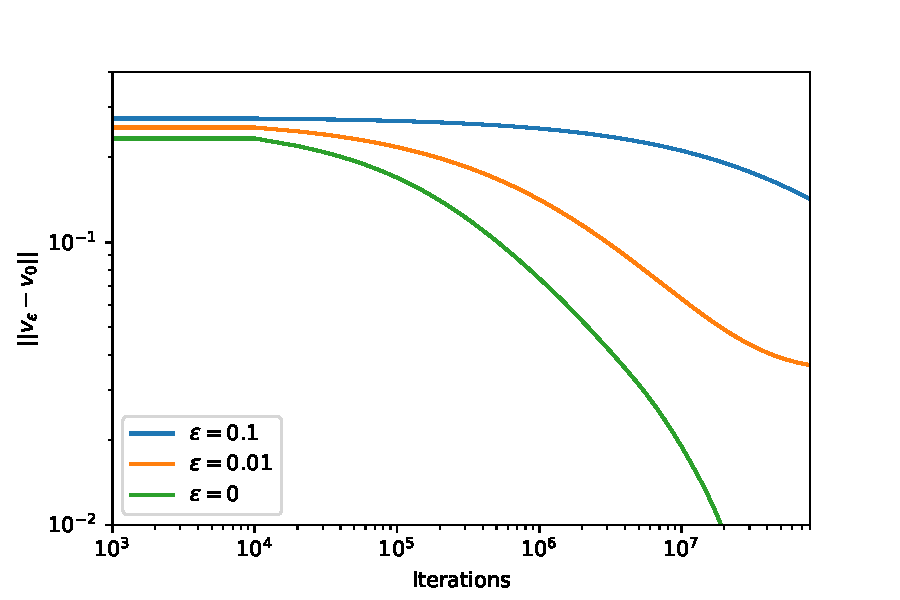
\includegraphics[width=\linewidth]{figures/semi_discrete_eps2.pdf}
        \caption{Convergence plot for several values of $\varepsilon$.}
    \end{subfigure}
    \caption{Another example of convergence for the French administrative region ``Bretagne''.}
    \label{fig:loire}
\end{figure}